\documentclass[12pt]{article}
%\usepackage[utf8]{inputenc}
%\documentclass[UTF8]{ctexart}
%\usepackage[UTF8, heading = false, scheme = plain]{ctex}
\usepackage{geometry}
%geometry{a4paper,scale=0.9}
\geometry{a4paper,left=1cm,right=1cm,top=1cm,bottom=2cm}
\usepackage{amsfonts}
\usepackage{color}
\usepackage{url}
%\usepackage{biblatex}
\usepackage{amsmath}
\usepackage{amssymb}
\usepackage{latexsym}
\usepackage{cite}
%\addbibresource{ref.bib}
%\bibliography{ref.bib}
\usepackage{caption}
\usepackage{graphicx, subfig}
\usepackage{float}
%\usepackage[fontset=ubuntu]{ctex}
%\usepackage{fontspec}
\usepackage{xeCJK}
%\usepackage[colorlinks,
%anchorcolor=black,
%citecolor=black]{hyperref}
%\setmainfont{SimSun}
\usepackage[section]{placeins}
\usepackage{enumitem}
\usepackage{framed}
\usepackage[framemethod=TikZ]{mdframed}
\usepackage{indentfirst}
\usepackage{setspace}%使用间距宏包
\linespread{1.5}
%\title{预备知识}
%\author{leolinuxer }
%\date{June 2020}

\title{共轭梯度法(Conjugate Gradient Method)\cite{Conjugate_Gradient_Method_No_Pain}}
\author{leolinuxer}
%\date{June 2020}

\begin{document}
%\setlength{\parindent}{0pt}
\maketitle
\tableofcontents
\section{背景和前置知识}
\subsection{CG 的适用场景}
CG(Conjugate Gradient,共轭梯度)算法是迭代式的算法,适用于求解如下形式的大规模线性方程组:
$$
Ax = b
$$
其中 $x$ 是未知向量,$b$是已知向量,$A$是已知的、对称的、正定的(或非正定)、方阵。

类似 CG 类的迭代式方法,适用于$A$是稀疏矩阵的情况。

上式的展开形式为:
$$
\begin{bmatrix}
A_{11} & A_{12} & \cdots & A_{1n} \\
A_{21} & A_{22} & \cdots & A_{2n} \\
\vdots & \vdots & \ddots & \vdots \\
A_{n1} & A_{n2} & \cdots & A_{nn} \\
\end{bmatrix}
\begin{bmatrix}
x_1 \\ x_2 \\ \vdots \\ x_n
\end{bmatrix} = 
\begin{bmatrix}
b_1 \\ b_2 \\ \vdots \\ b_n
\end{bmatrix}
$$

\subsection{内积}
两个向量 $x, y$ 的内积记作:$x^Ty$,表示对应元素的乘积和:$\sum_{i=1}^nx_iy_i$。

向量的内积满足:
$$
x^Ty = y^Tx
$$

如果 $x$ 和 $y$ 正交,则 $x^Ty = 0$。

\subsection{正定矩阵}
如果对于任意非零向量 $x$,都有:
$$
x^TAx \ge 0
$$
则称$A$为正定矩阵。

\subsection{矩阵的性质}
$$
(AB)^T = B^TA^T
$$
$$
(AB)^{-1} = B^{-1}A^{-1}
$$

\section{特征值和特征向量}
\subsection{特征向量的性质}
给定矩阵 $B$ 的特征向量 $v$,二者的乘积 $Bv$ 只会对 $v$ 形成比例变化(或反向比例变化),而不会形成旋转变化,也就是说 $Bv$ 满足: $Bv = \lambda v$,其中 $\lambda$ 是特征值。

对于任意常量 $\alpha$,向量 $\alpha v$ 也是 $B$ 的特征向量,特征值同样为 $\lambda$。这是因为 $B(\alpha v) = \alpha Bv = \lambda (\alpha v)$。

为什么需要回忆特征向量的知识点呢,这是因为迭代的方法通常都涉及到进行反复的矩阵-向量运算。当矩阵 $B$ 反复作用于特征向量 $v$ 后,会发生如下情况:
\begin{itemize}
\setlength{\itemsep}{0pt}
\setlength{\parsep}{0pt}
\setlength{\parskip}{0pt}
    \item 如果 $|\lambda| < 1$,那么 $B^i v = \lambda^i v$,当 $i$ 趋近于无穷大时,$B^i v$ 会逐渐趋于0(如图9所示);
    \item 如果 $|\lambda| > 1$,那么 $B^i v = \lambda^i v$,当 $i$ 趋近于无穷大时,$B^i v$ 会逐渐趋于无穷大(如图10所示);
\end{itemize}
\begin{figure}[H]
    \centering
    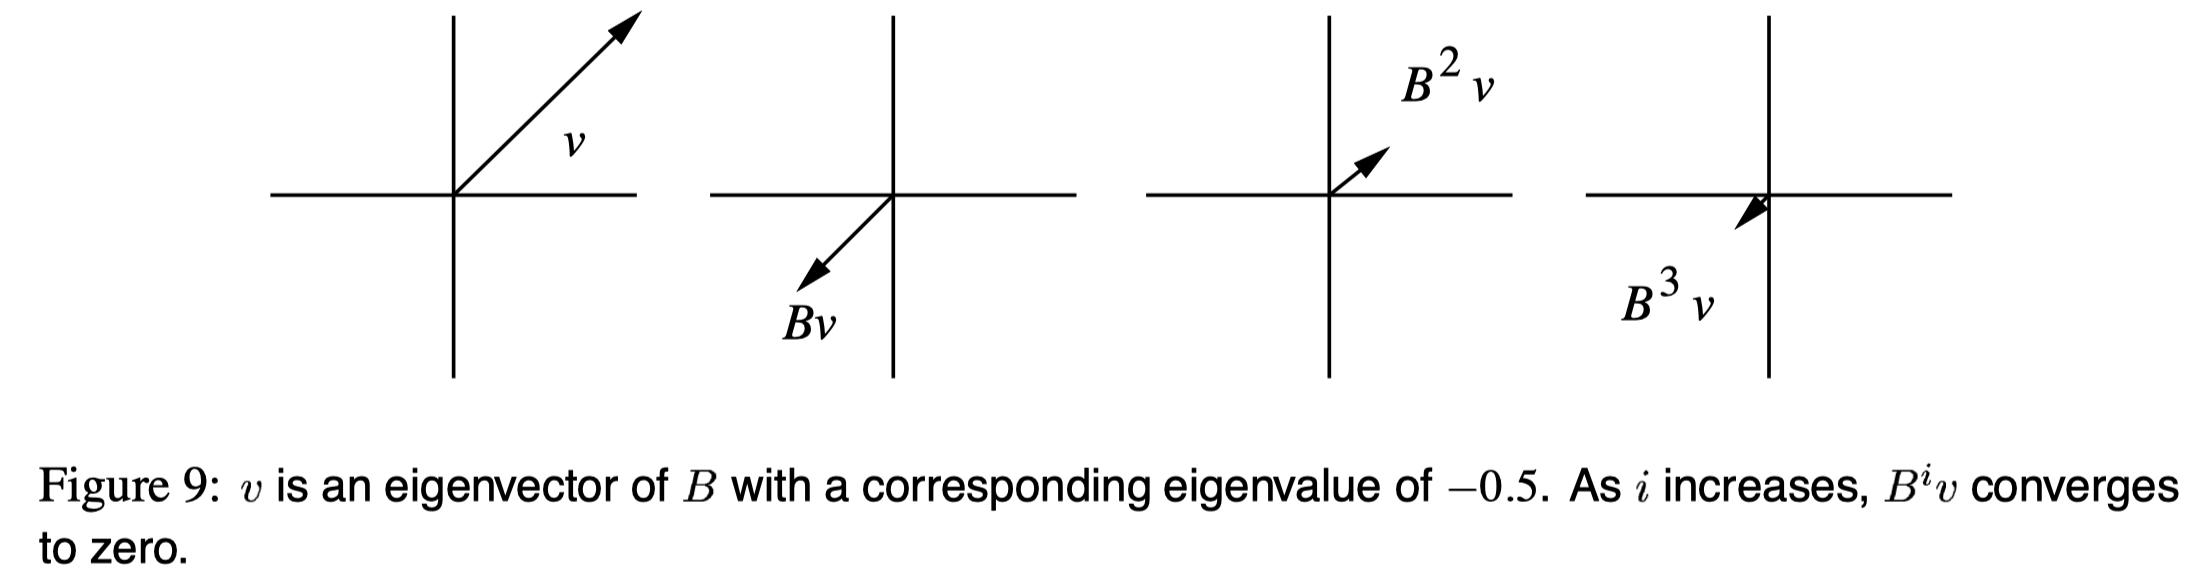
\includegraphics[width=1\textwidth]{fig/CG_Plot_Eightvalue_1.png}
\end{figure}
\begin{figure}[H]
    \centering
    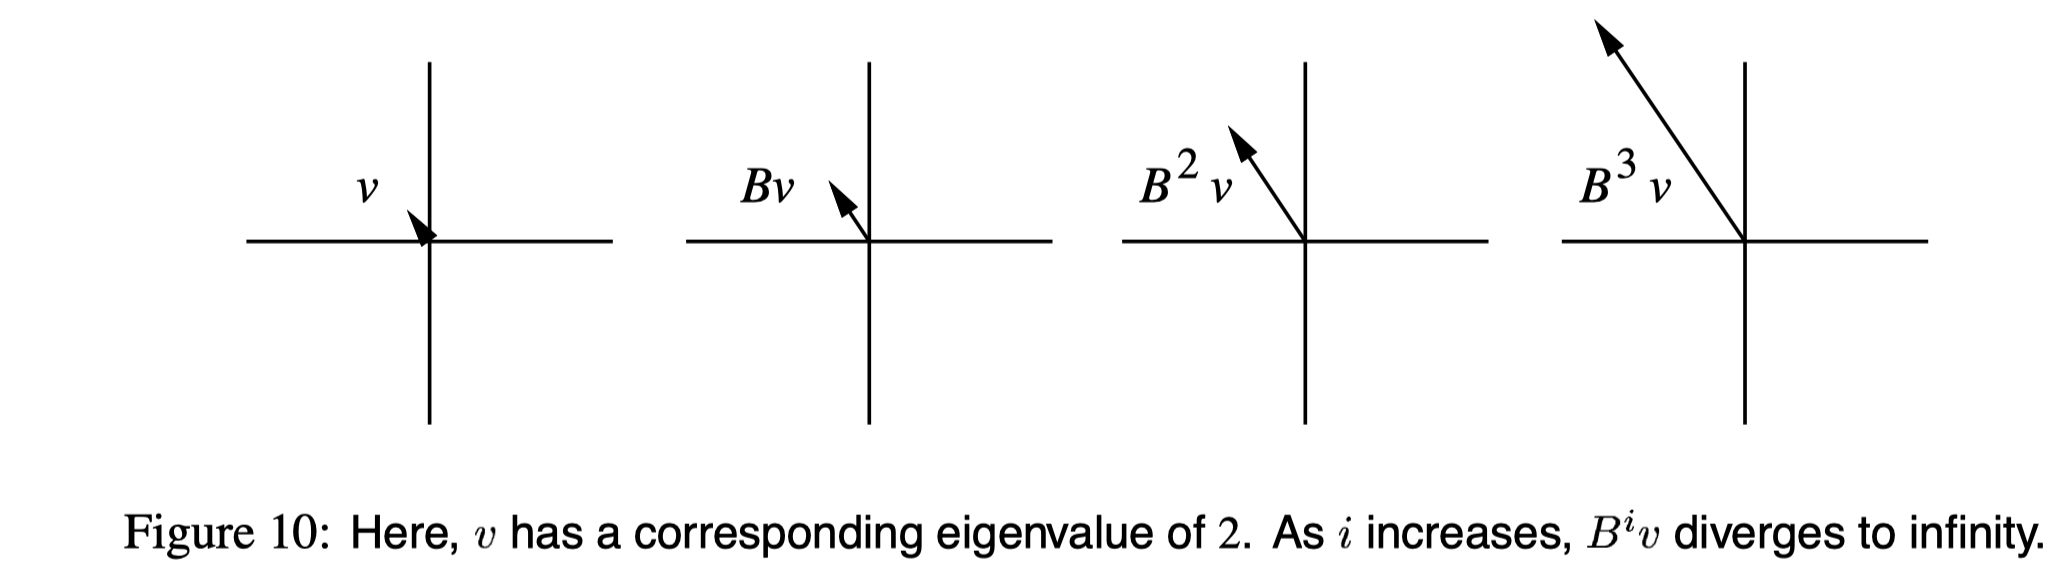
\includegraphics[width=1\textwidth]{fig/CG_Plot_Eightvalue_2.png}
\end{figure}

\textbf{如果 $B$ 是对称矩阵,那么 $B$ 存在 $n$ 个线性无关的特征向量 $v_1, v_2, \cdots, v_n$}(注意不是唯一集合,因为特征向量可以进行比例变换)和对应的 $n$ 个特征值 $\lambda_1, \lambda_2, \cdots, \lambda_n$(特征值是唯一的,特征值间可以相等,也可以不等)。

\begin{framed}
\textbf{证明:$n$维对称矩阵有 $n$ 个正交的特征向量}

首先,\textbf{任意矩阵都至少有一个特征向量}。原因是,给定矩阵$A$ ,那么 $\text{det}(A - \lambda I)$ 是关于 $\lambda$ 的多项式,至少有1个解(可能为复数),记作 $\lambda_A$。所以行列式 $A - \lambda_AI = 0$,因此矩阵 $A - \lambda_AI$ 是奇异的,因此必有非零向量 $v$ 使得 $(A - \lambda_AI)v = 0$。那么有 $Av = \lambda_Av$,所以向量 $v$ 是 $A$ 的特征向量。

接下来,证明任意对称矩阵都有 $n$ 个正交的特征向量。举一个 $4 \times 4$ 的矩阵 $A$ 为例,它至少有一个特征值 $\lambda_A$ 和对应的特征向量 $v$。令 $x_1 = v / ||v||$( $x_1$ 有单位长度),通过 Gram-Schmidt orthogonalization 方法,可以得到互相正交的三个单位向量 $x_2, x_3, x_4$。定义 $X = [x_1, x_2, x_3, x_4]$,因为 $x_i$ 互相是正交的,所以 $X^TX = I, X^T = X^{-1}$。

注意到,对于任意 $i \neq 1$,有 $x_1^TAx_i = (x_1^TAx_i)^T = x_i^TA^Tx_1 = x_i^TAx_1  =  x_i^T \lambda_Ax_1 = 0$,所以:
\begin{align*}
X^TAX &= \begin{bmatrix}x_1^T \\ x_2^T \\ x_3^T \\ x_4^T \end{bmatrix} A \begin{bmatrix}x_1 & x_2 & x_3 & x_4 \end{bmatrix} =  \begin{bmatrix}x_1^T \\ x_2^T \\ x_3^T \\ x_4^T \end{bmatrix} \begin{bmatrix} \lambda_Ax_1 & Ax_2 & Ax_3 & Ax_4 \end{bmatrix} \\
           &= 
\begin{bmatrix}
\lambda_A & 0 & 0 & 0 \\
0 & & & \\
0 & & B & \\
0 & & & \\
\end{bmatrix}
\end{align*}

其中,$B$ 是 $3 \times 3$ 的对称矩阵;$B$ 一定有特征向量 $\omega$ 和特征值 $\lambda_B$。定义 $\hat{\omega}$ 为 长度为 4 的向量,其第一个元素为0,剩余元素为 $w$ 的元素;显然:
$$
X^{-1}AX\hat{\omega} = X^TAX\hat{\omega} = \begin{bmatrix}
\lambda_A & 0 & 0 & 0 \\
0 & & & \\
0 & & B & \\
0 & & & \\
\end{bmatrix} \hat{\omega} = \lambda_B\hat{\omega}
$$

换句话说,$AX\hat{\omega} = \lambda_BX\hat{\omega}$,所以 $X\hat{\omega}$ 是 $A$ 的特征向量。并且,$x_1^TX\hat{\omega} = [1 \ 0 \ 0 \  0]\hat{\omega} = 0$,所以 $x_1$ 和 $X\hat{\omega}$ 是正交的。所以 $A$ 至少有两个互相正交的特征向量。

递归可以证明,$A$ 的所有特征向量都是两两正交的。
\end{framed}
 
\subsection{谱半径}
因为对称矩阵 $B$ 的 $n$ 个特征向量是线性无关的,所以\textbf{这组特征向量构成了空间 $\mathbb{R}^n$ 的一组正交基}。所以,当 $B$ 与非特征向量 $x$ 进行乘法时,可以把 $x$ 用它的特征向量进行表示,然后分别观察在各个基上结果的变化。如图11所示,给定向量 $x$,将其表示为两个基向量 $v_1, v_2$ 的和。那么 $Bx = B(v_1 + v_2) = Bv_1 + Bv_2$,所以 $B^ix = B^iv_1 + B^iv_2 = \lambda^i_1 v_1 + \lambda^i_2 v_2$。如果所有的特征值都小于1,那么 $B^ix$会趋近于0;如果至少有一个特征值大于1,那么 $B^ix$ 会趋近于无穷大。由此引出了矩阵的 \textbf{谱半径(spectral radius)}:
 $$
 \rho (B) = \max|\lambda_i|, \qquad \lambda_i\text{是} B \text{的特征向量}
 $$
 
 如果期望 $B^ix$ 迅速趋近于0,那么 $rho(B) < 1$,并且越小越好。
 \begin{figure}[H]
    \centering
    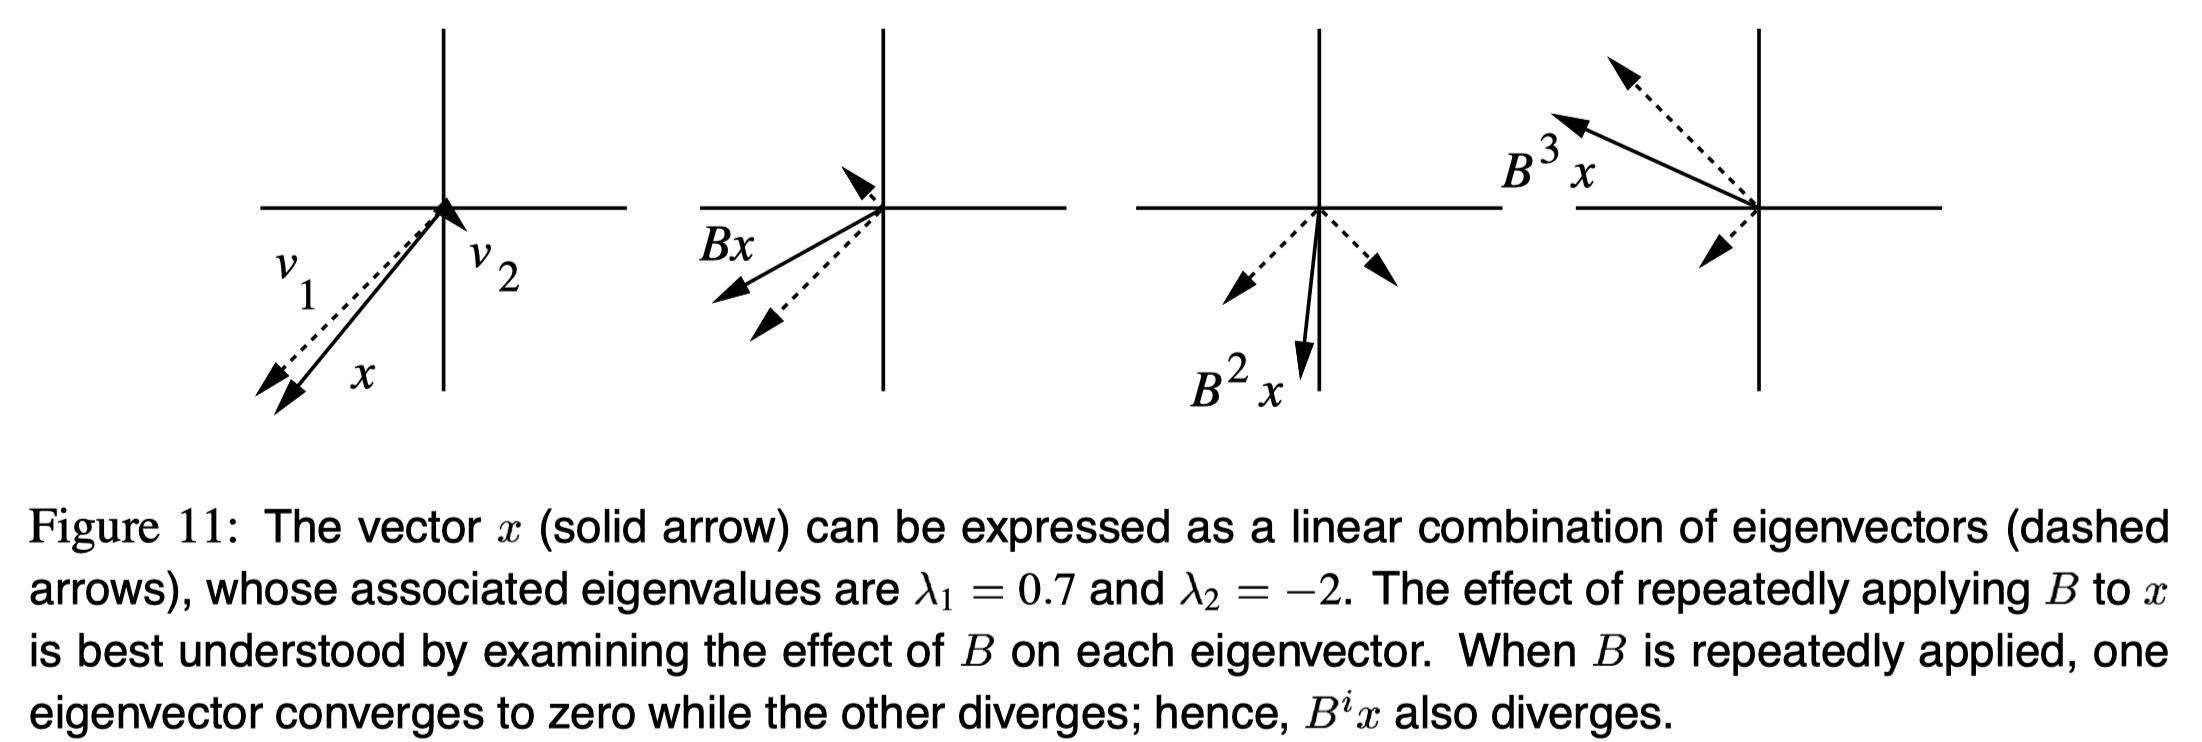
\includegraphics[width=1\textwidth]{fig/CG_Plot_Eightvalue_3.png}
\end{figure}

 \subsection{正定矩阵的特征值}
 \textbf{正定矩阵的特征值均大于0},证明如下
\begin{align*}
Bv &= \lambda v \\
v^T B v &= \lambda v^T v
\end{align*}

因为 $B$ 是正定矩阵,所以对于任意非零向量 $v$ 都有 $v^T B v > 0$,所以必有 $\lambda > 0$。
 
\subsection{一个具体的例子}
给定矩阵 $A$,它的特征向量 $v$ 和特征值 $\lambda$ 满足:
$$
Av = \lambda v = \lambda Iv \Rightarrow (\lambda I - A) v = 0
$$

因为 $v$ 是非零向量,所以 det($\lambda I - A) = 0$,以后文会用到的 $A = \begin{bmatrix}3 & 2 \\ 2 & 6\end{bmatrix}$ 为例,有:
$$
\text{det}\begin{bmatrix}
\lambda - 3 & -2 \\ -2 & \lambda -6
\end{bmatrix} = \lambda^2 - 9\lambda + 14 = (\lambda - 7)(\lambda - 2)
$$

所以,特征是是 $\lambda_1 = 7, \lambda_2 = 2$。当 $\lambda_1 = 7$ 时,有:
$$
(\lambda I - A) v = \begin{bmatrix}4 & -2 \\ -2 & 1\end{bmatrix}\begin{bmatrix}v_1 \\ v_2 \end{bmatrix} = 0
$$
$$
\therefore 4v_1 - 2v_2 = 0
$$

任意满足该方程的解都可以构成对应的特征向量,比如 $v = [1, 2]^T$。同理,可以求得特征值 $\lambda_2 = 2$ 对应的特征向量为$v = [-2, 1]^T$。如下图所示,$A$ 的两个特征向量对应了图中的两个箭头,并且较大的特征值 $\lambda_1 = 7$ 对应了更陡的斜率。

\begin{figure}[H]
    \centering
    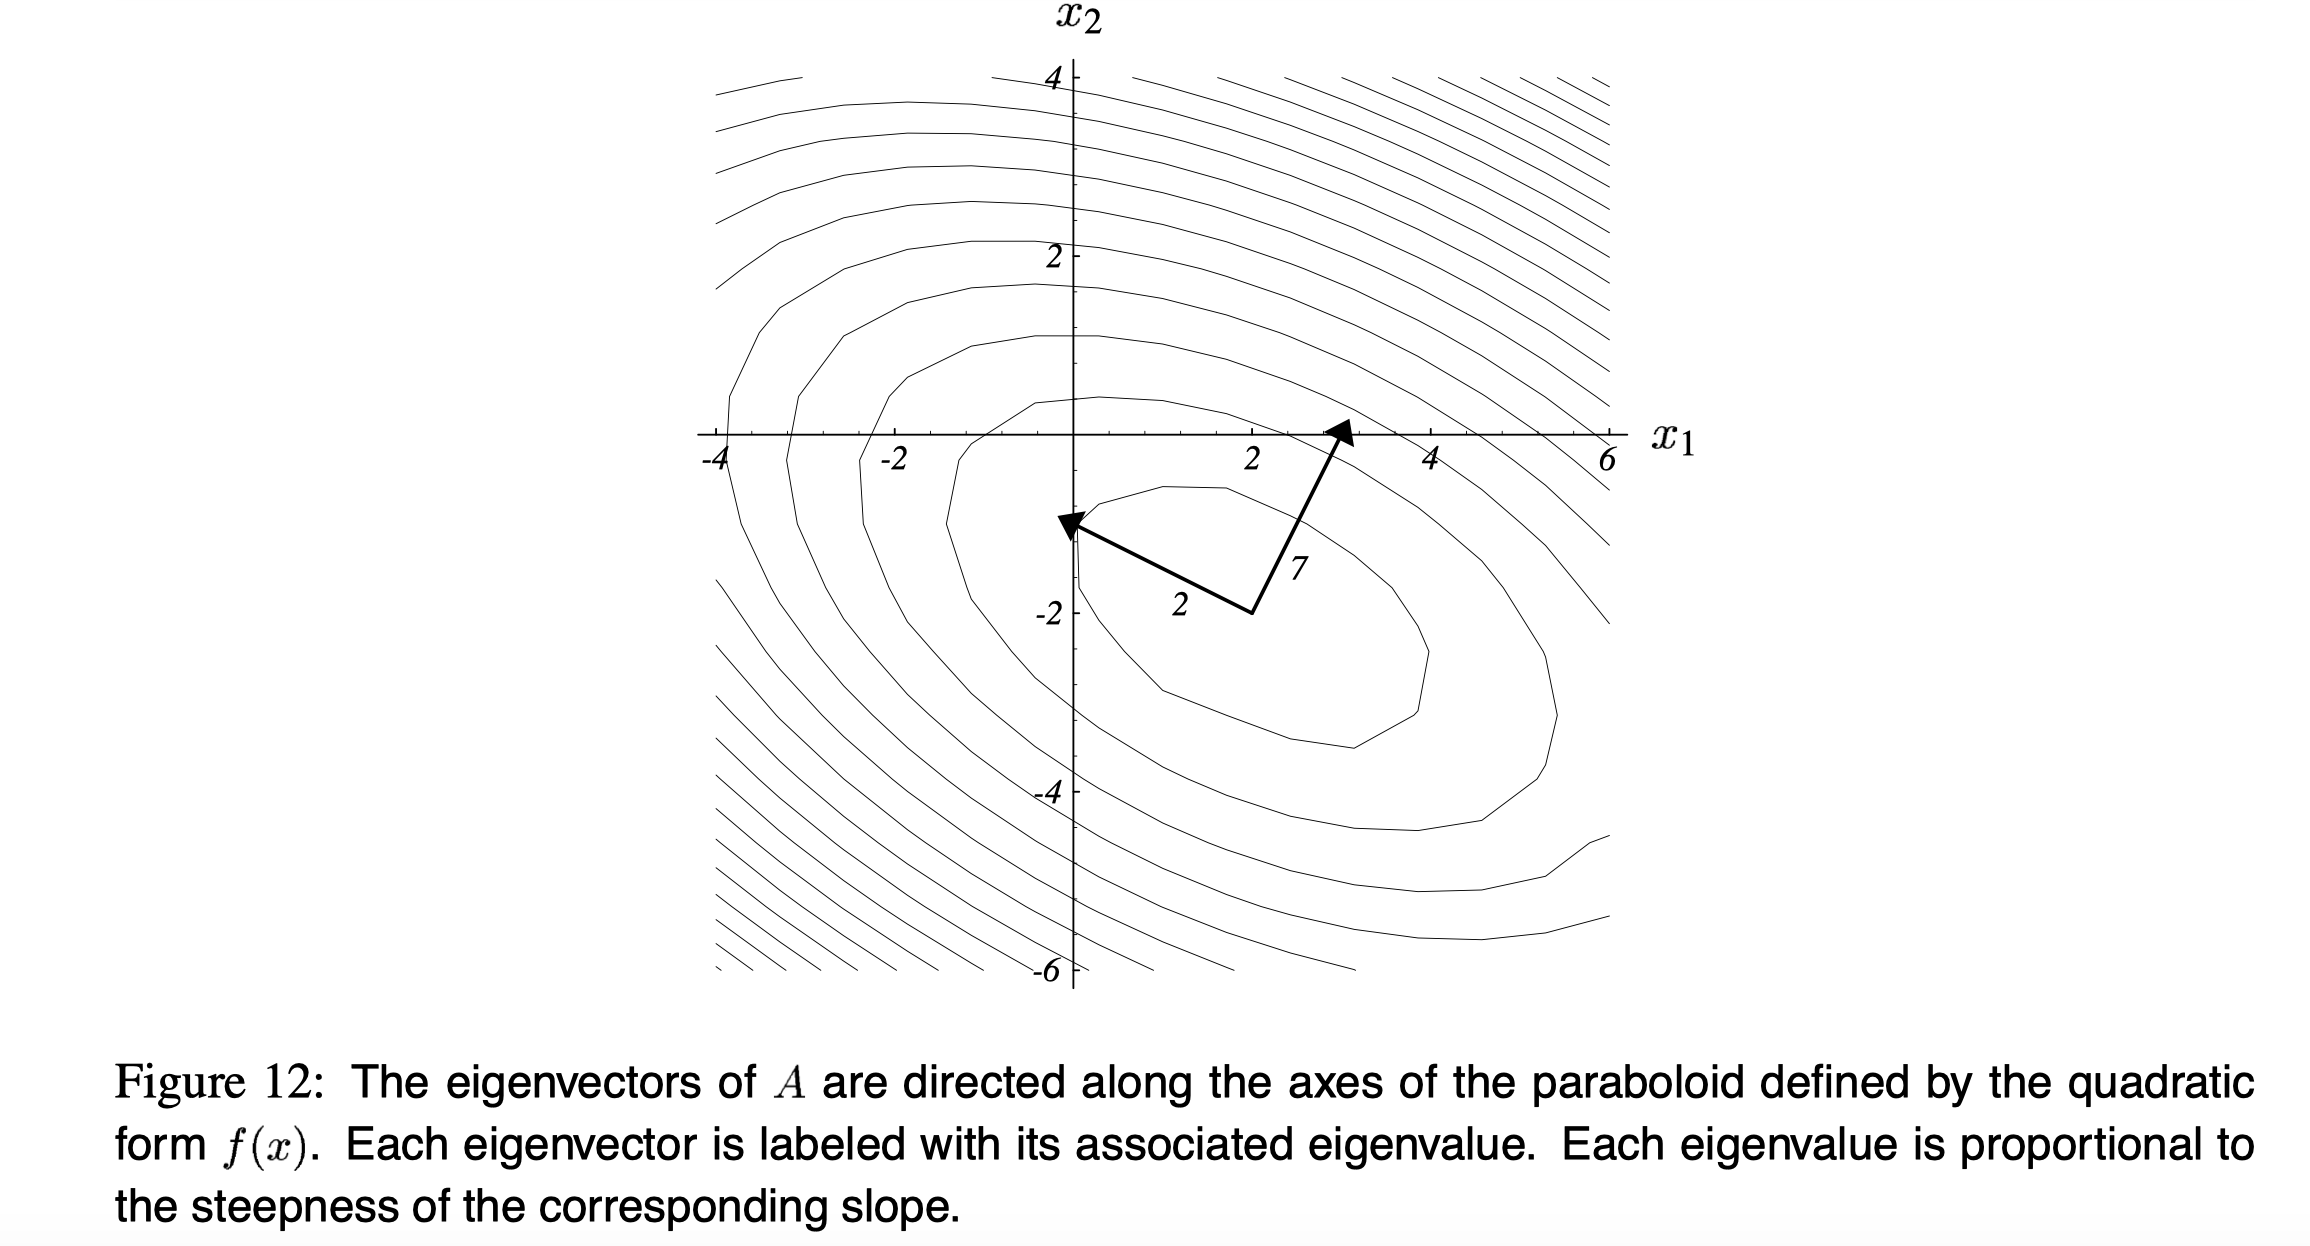
\includegraphics[width=1\textwidth]{fig/CG_Plot_Eightvalue_4.png}
\end{figure}

\section{二次型(Quadratic Form)}
向量的二次型形式为:
$$
f(x) = \frac{1}{2}x^TAx - b^Tx + c
$$
其中 $A$ 是矩阵,$b$ 和 $x$ 是向量,$c$ 是常量。

\textbf{如果 $A$ 是对称正定阵,那么 当 $Ax = b$ 时,$f(x)$ 取得最小值}。

\subsection{一个具体的例子}
$$
A = \begin{bmatrix} 3 & 2 \\ 2 & 6 \end{bmatrix} \qquad 
b = \begin{bmatrix} 2 \\ -8 \end{bmatrix} \qquad 
c = 0
$$

$Ax = b$ 的图像如下:
\begin{figure}[H]
    \centering
    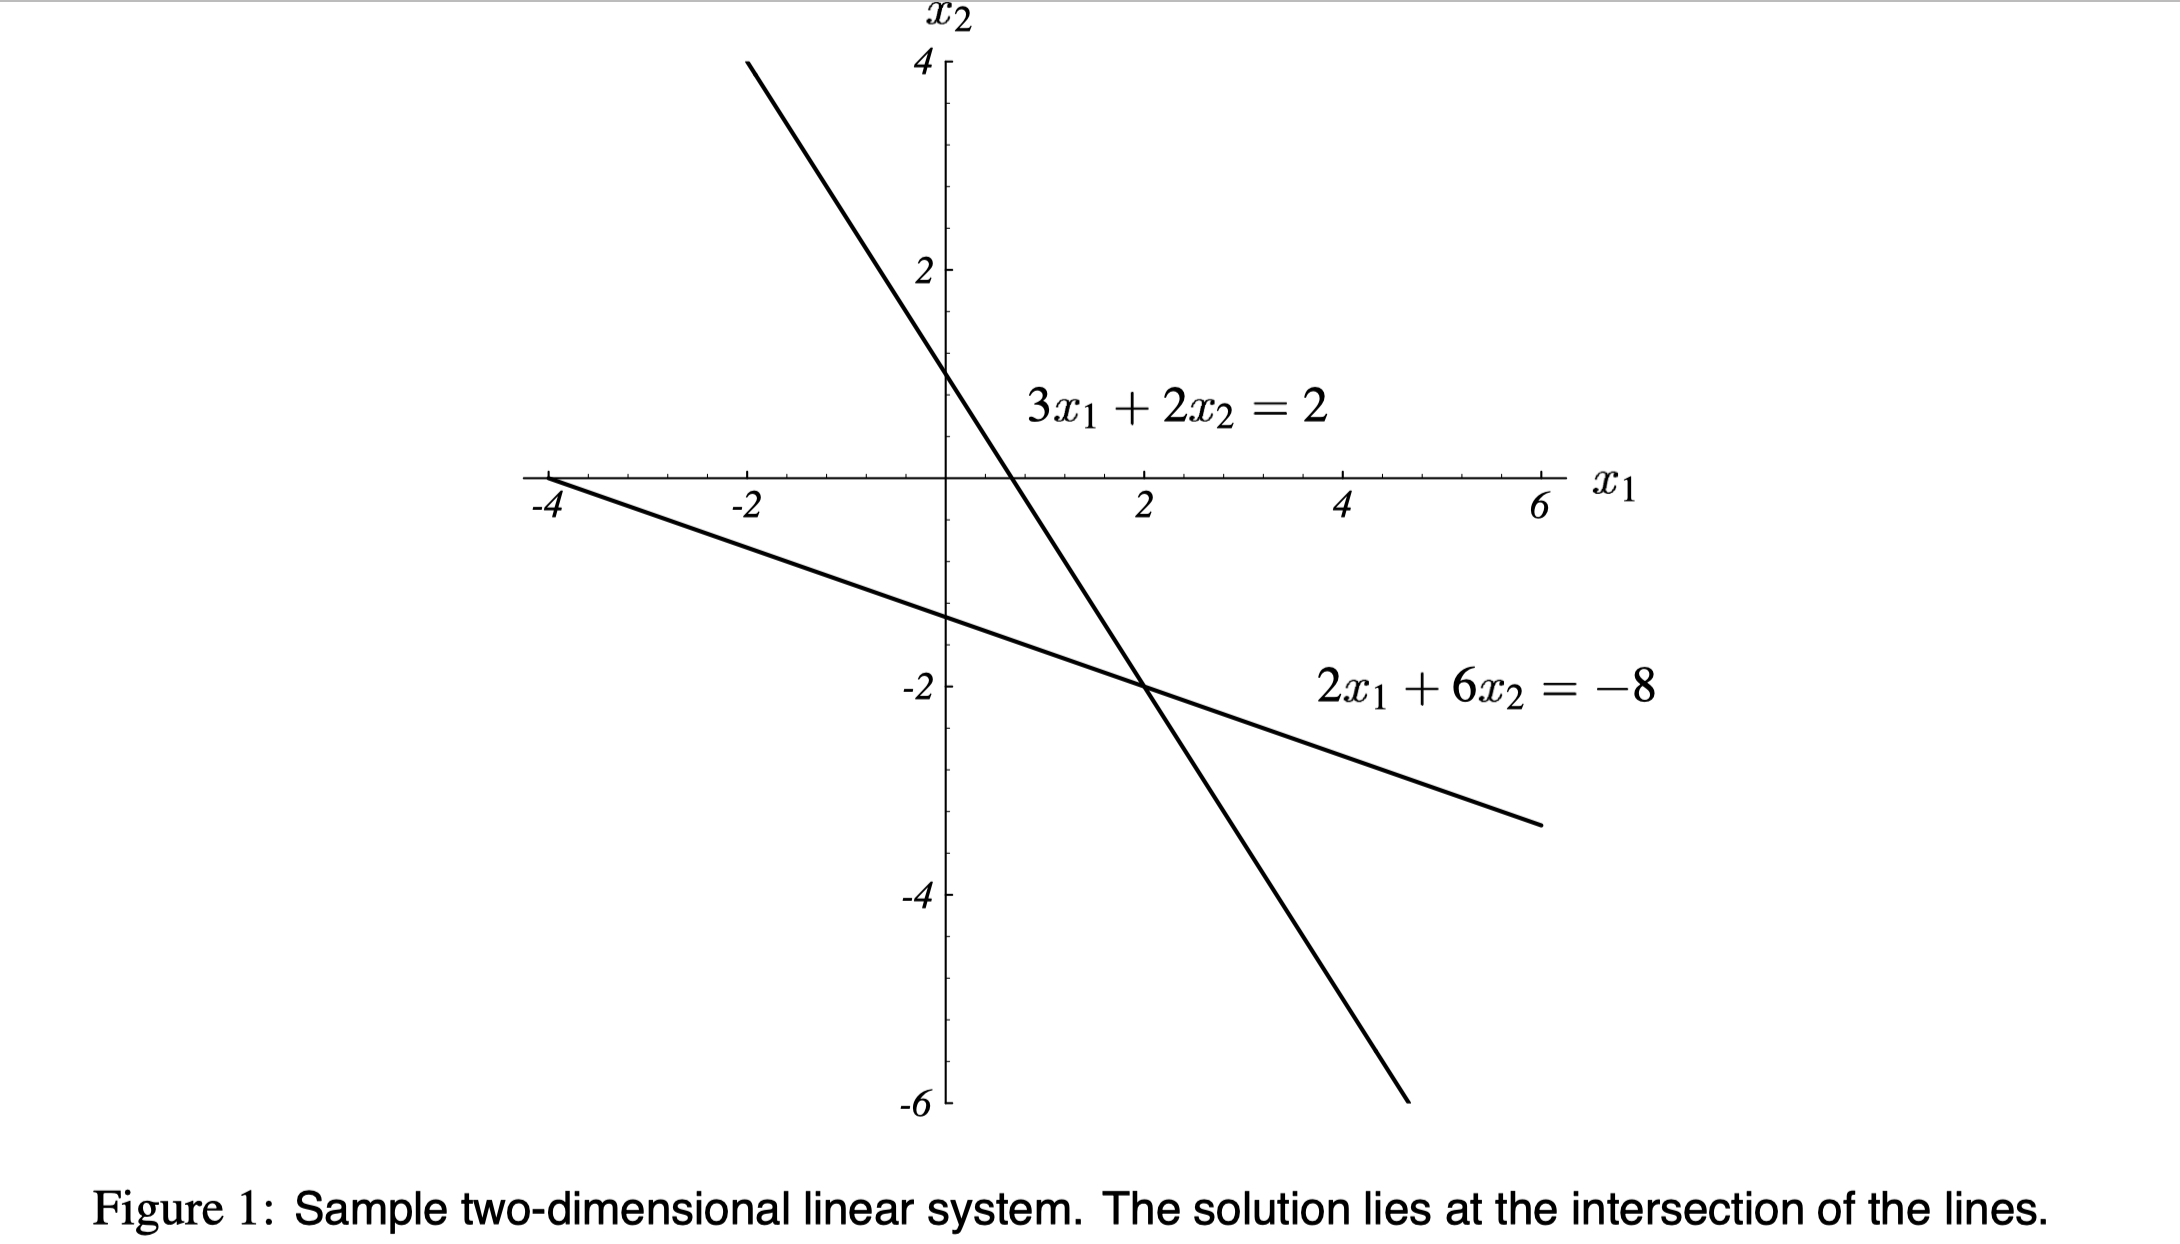
\includegraphics[width=.8\textwidth]{fig/CG_Plot_Eq_1.png}
\end{figure}
方程的解位于 $n=2$ 维超平面的交点处,每个超平面有 $n-1=1$ 维。本方程的解为 $x = [2, -2]^T$;

对应的二次型 $f(x)$ 的图像为:
\begin{figure}[H]
    \centering
    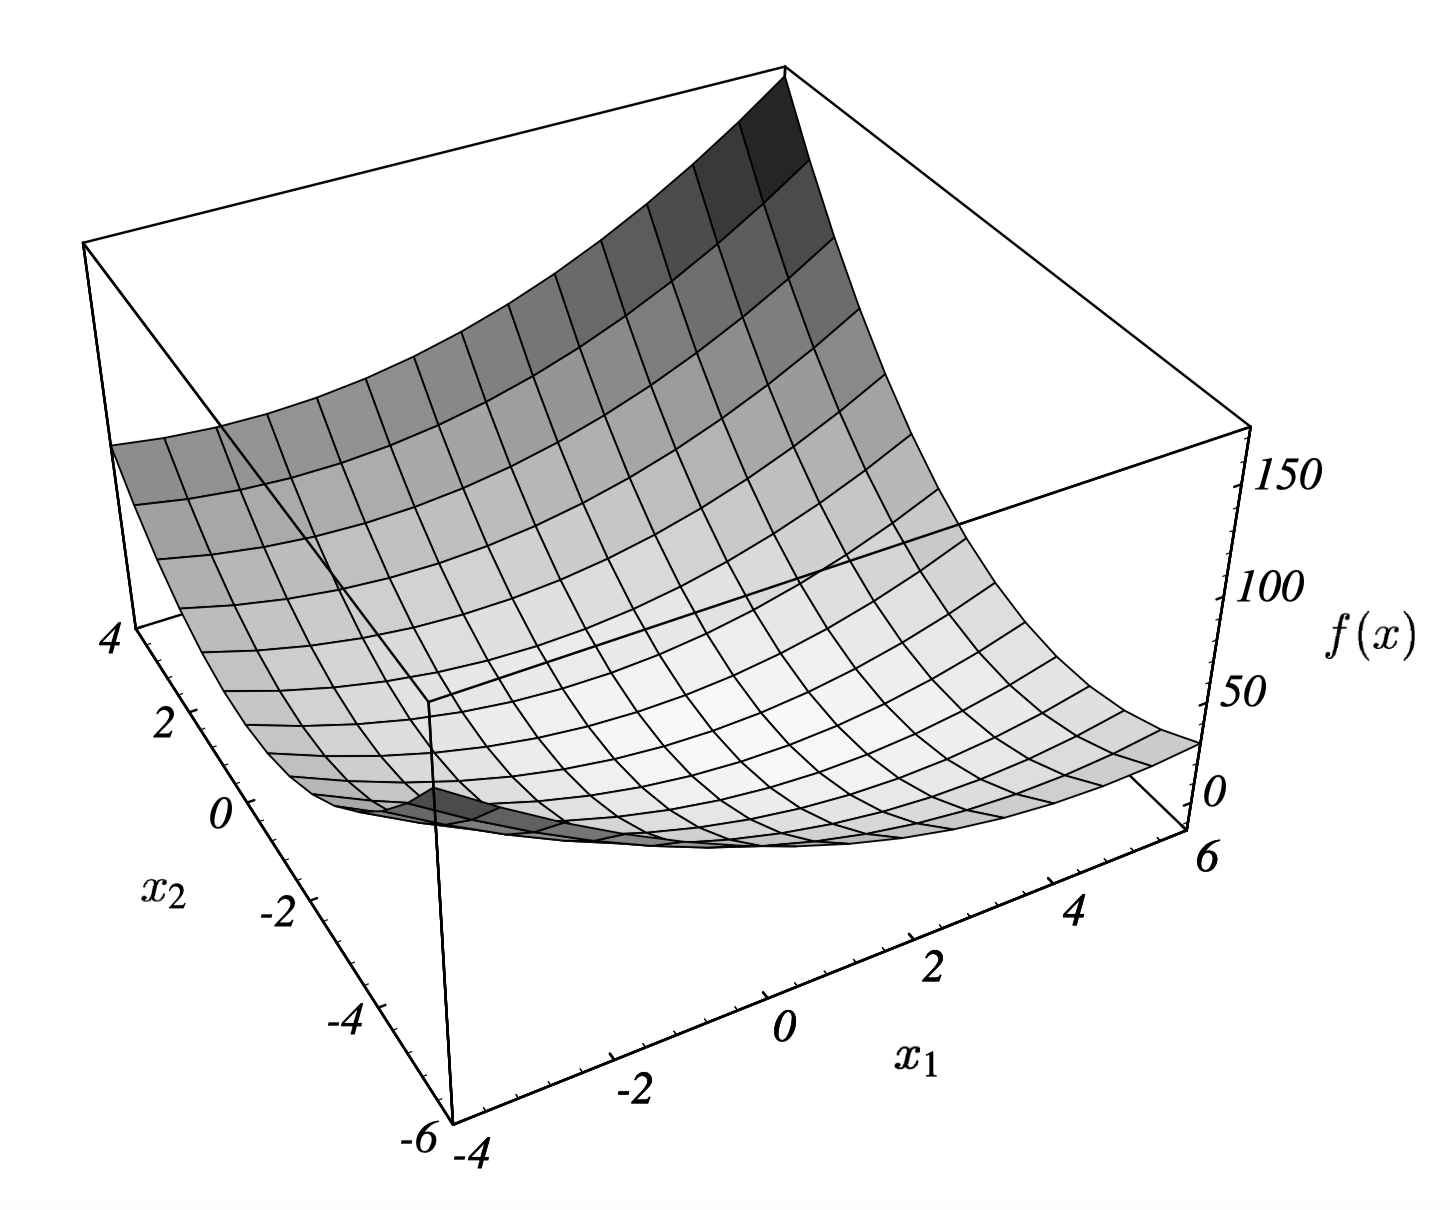
\includegraphics[width=.6\textwidth]{fig/CG_Plot_Eq_2.png}
\end{figure}

它的等高线图如下:
\begin{figure}[H]
    \centering
    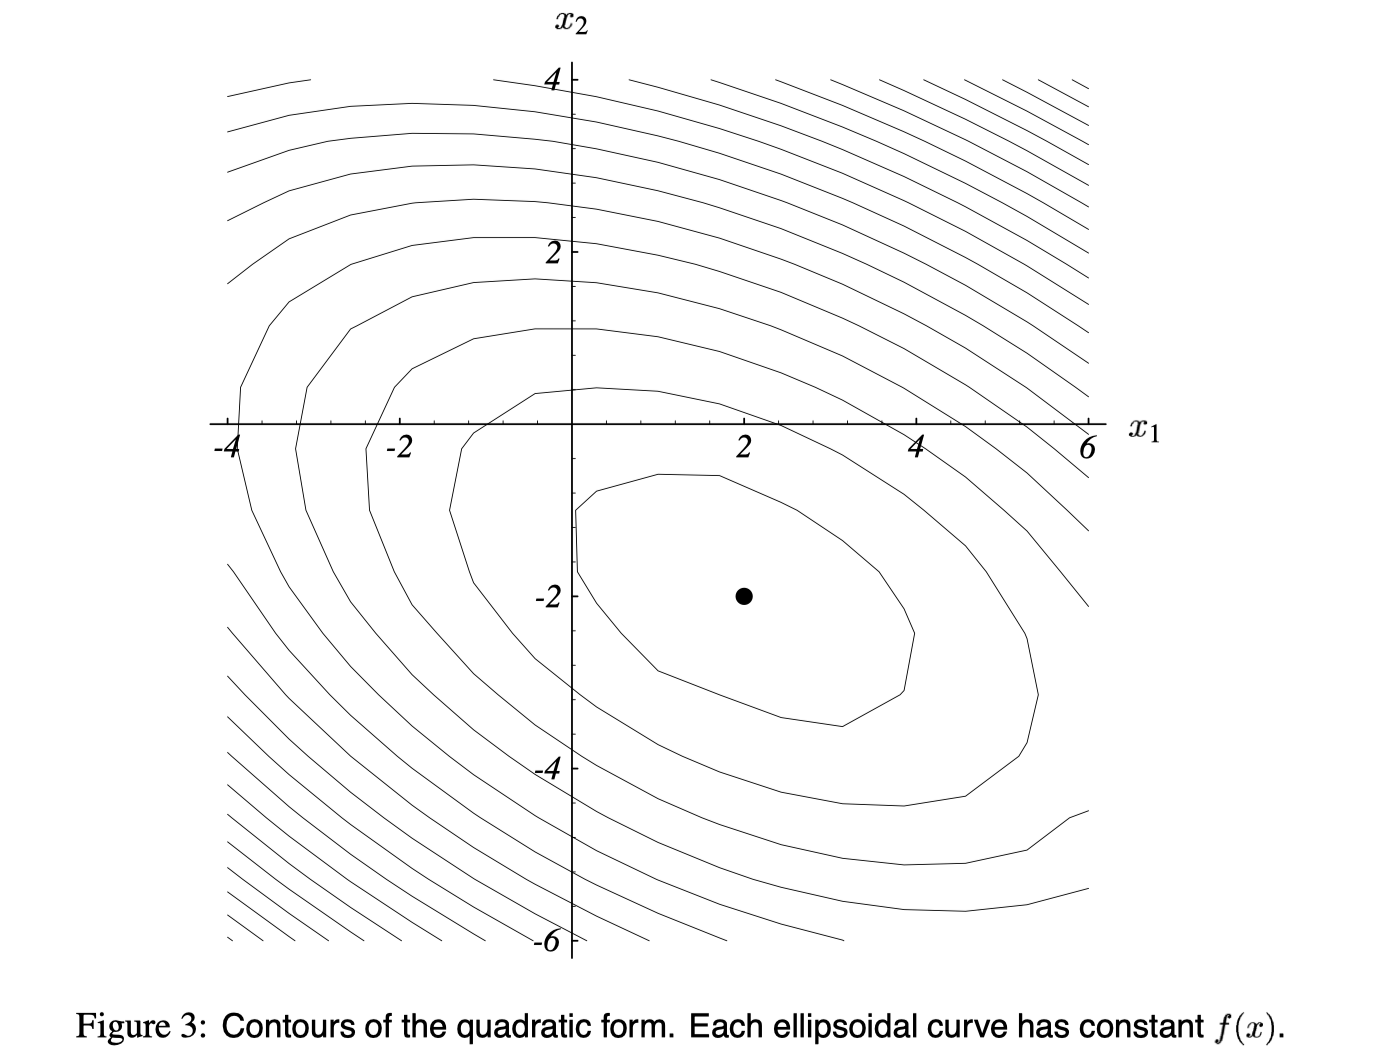
\includegraphics[width=.6\textwidth]{fig/CG_Plot_Eq_3.png}
\end{figure}

因为 $A$ 是正定矩阵,所以 $f(x)$ 的形状为抛物面形。

\subsection{梯度向量}
$f(x)$ 的梯度为:
$$
f'(x) = \begin{bmatrix}
\frac{\partial}{\partial x_1}f(x) \\
\frac{\partial}{\partial x_2}f(x) \\
\vdots \\
\frac{\partial}{\partial x_n}f(x) \\
\end{bmatrix}
$$

上面例子的梯度向量如下图所示:
\begin{figure}[H]
    \centering
    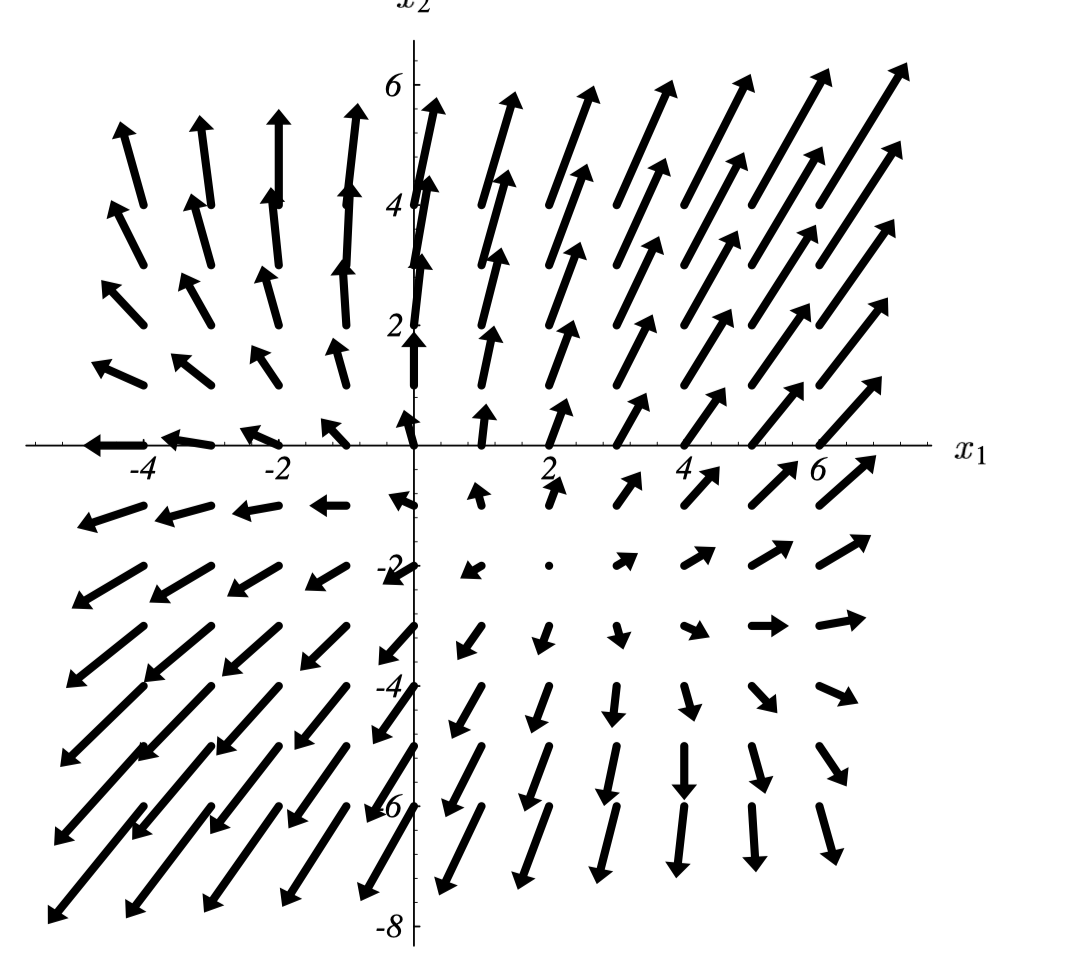
\includegraphics[width=.4\textwidth]{fig/CG_Plot_Eq_4.png}
\end{figure}
当 $f'(x) = 0$ 时,$f(x)$ 可以取得最小值。

根据$f(x) = \frac{1}{2}x^TAx - b^Tx + c$ ,有:
$$
f'(x)  = \frac{1}{2}A^Tx + \frac{1}{2}Ax - b
$$

如果 $A$ 是对称矩阵,那么有
$$
f'(x) = Ax - b
$$

所以,当 $f'(x) = Ax - b = 0$ 时,$f(x)$ 有最小值。也就是说,$Ax=b$的解是 $f(x)$ 的 critical point。如果 $A$ 是正定对称阵,那么$Ax=b$ 的解对应 $f(x)$  的最小值;

如果 $A$ 不是对称阵,那么根据$f'(x) = 0$ 有:$\frac{1}{2}(A^T+A)x = b$,并且 $\frac{1}{2}(A^T+A)$ 是对称的。

\subsection{进一步解释}
根据 $f(x) = \frac{1}{2}x^TAx - b^Tx + c$,我们可以知道如果 $A$ 是对称阵(无论是否正定),对于任意点 $p$ 和 $x = A^{-1}b$,都有:
$$
f(p) = f(x) + \frac{1}{2}(p-x)^TA(p-x)
$$

如果 $A$ 是正定的,那么根据正定矩阵的性质,对于任意$p \neq x$,都有 $\frac{1}{2}(p-x)^TA(p-x) > 0$,所以 $p = x$ 是 $f(x)$ 的最小值解。

\begin{framed}
\textbf{证明:如果 $A$ 是对称正定阵,那么 $Ax=b$ 的解最小化二次型}

假定 $A$ 是对称阵,$e$ 是误差项,那么有:
\begin{align*}
f(x+e) &= \frac{1}{2}(x+e)^TA(x+e) - b^T(x+e) + c \\
	  &= \frac{1}{2}x^TAx + e^TAx + \frac{1}{2}e^TAe - b^Tx - b^Te + c \\
	  &= \frac{1}{2}x^TAx - b^Tx + c + e^Tb + \frac{1}{2}e^TAe - b^Te \\
	  &= f(x) + \frac{1}{2}e^TAe
\end{align*}

如果 $A$ 同时也是正定的,那么对于任意 $e \neq 0$,都有 $\frac{1}{2}e^TAe > 0$;所以,$x$ 是 $f(x)$ 的最小值解。证毕。

进而,假定 $p = x + e$,即 $e = p - x$,那么有:
\begin{align*}
f(p) &= f(x + e) \\
      &= f(x) + \frac{1}{2}e^TAe \\
      &= f(x) + \frac{1}{2}(p-x)^TA(p-x)
\end{align*}
\end{framed}

不同 $A$ 的正定情况,对应着不同的图像如下:
\begin{figure}[H]
    \centering
    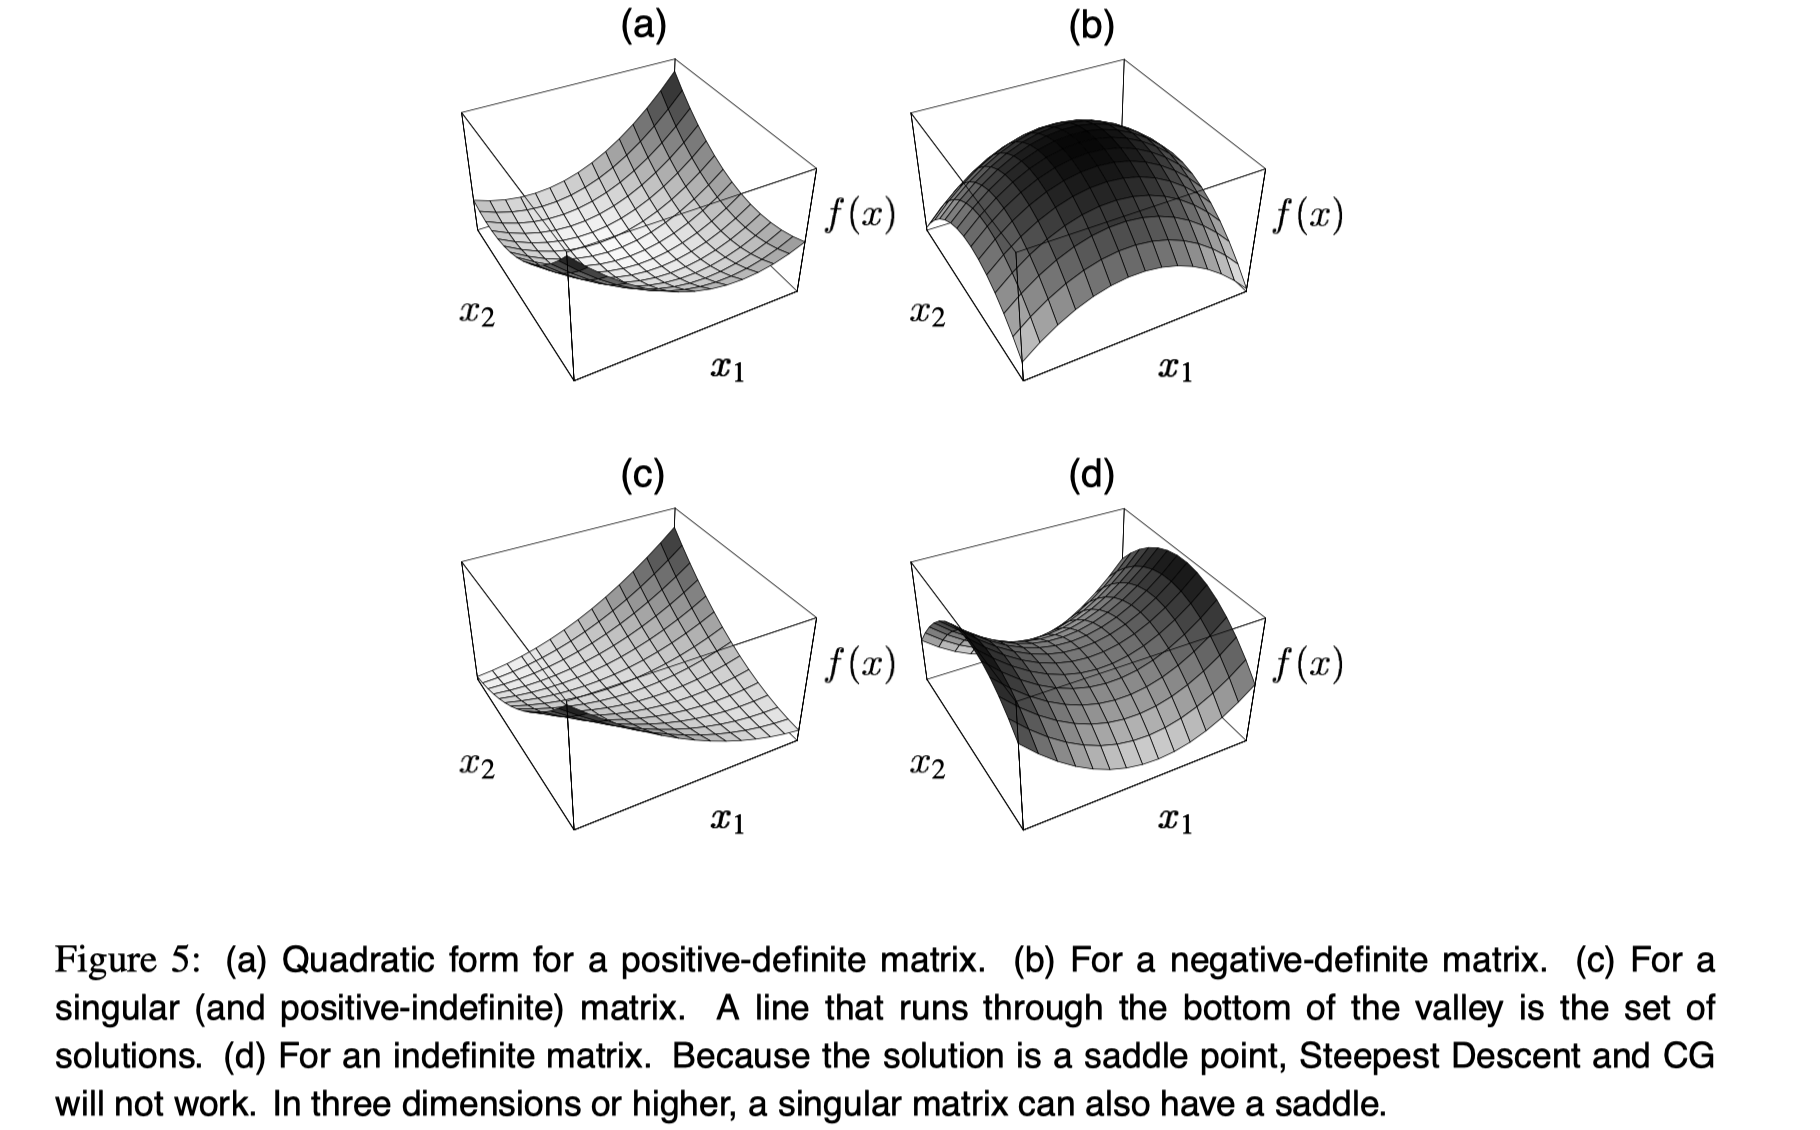
\includegraphics[width=1\textwidth]{fig/CG_Plot_Eq_5.png}
\end{figure}

\section{最速下降法(Steepest Descent)}
\subsection{最速下降法过程推导}
最速下降法:从任意点 $x_0$ 出发,沿着梯度下降,途经点为 $x_1, x_2, \cdots $ 直到足够接近解 $x$。其中,每次下降都选择 $f$ 下降最快的方向,也就是 $f'(x_i)$ 的反方向。因为 $f(x_i) = \frac{1}{2}x_i^TAx_i - b^Tx_i + c$,$f'(x_i) = Ax_i - b$,所以下降的方向是:$-f'(x_i) = -Ax_i + b$。

定义如下符号:
\begin{itemize}
\setlength{\itemsep}{0pt}
\setlength{\parsep}{0pt}
\setlength{\parskip}{0pt}
    \item 误差 $e_i = x_i - x$,表示 $x_i$ 与 $x$ 的接近程度;
    \item 余量$r_i = b - Ax_i$,表示 $Ax_i$ 与 $b$ 的接近程度;显然,有:$r_i = -Ae_i$,所以可以把 $r_i$ 想象为误差 $e_i$ 经过矩阵 $A$ 变换后得到的量。同时,显然有 $r_i = -f'(x_i)$,也就是说 $r_i$ 就是最速下降的方向。
\end{itemize}

假定从 $x_0 = [-2, -2]^T$ 出发,沿着最速下降方向(图6(a)的实线方向)前进,到达:
$$
x_1 = x_0 + \alpha r_0
$$

其中 $\alpha$ 是前进的步长,那么,应该向前走多远呢?

可以采用线搜索(line search)的方法,寻找到能够使得沿着该方向前进后,$f$ 取得最小值的最佳 $\alpha$。如图6(b)所示,垂直的平面是最速下降的方向,需要找到该平面和抛物面的交点。图6(c)是相交得到的抛物线(注意,横轴为 $\alpha$,纵轴为 $f(x_i + \alpha r_i))$;那么,该如何确定 $\alpha$ 呢,其实就是要找到该抛物线的最低点。

显然,当 $\frac{d}{d\alpha}f(x_1) = 0$ 时,能够求得 $f$ 的最小值。根据链式法则,有:
$$
\frac{d}{d\alpha}f(x_1) = f'(x_1)^T\frac{d}{d\alpha}x_1 =  f'(x_1)^T\frac{d}{d\alpha}(x_0 + \alpha r_0) =  f'(x_1)^Tr_0
$$

令该式为 0,即 $f'(x_1)^Tr_0 = 0$,也就是说,\textbf{此时 $f'(x_1)$ 与 $r_0$ 正交},如图6 (d) 所示。
\begin{figure}[H]
    \centering
    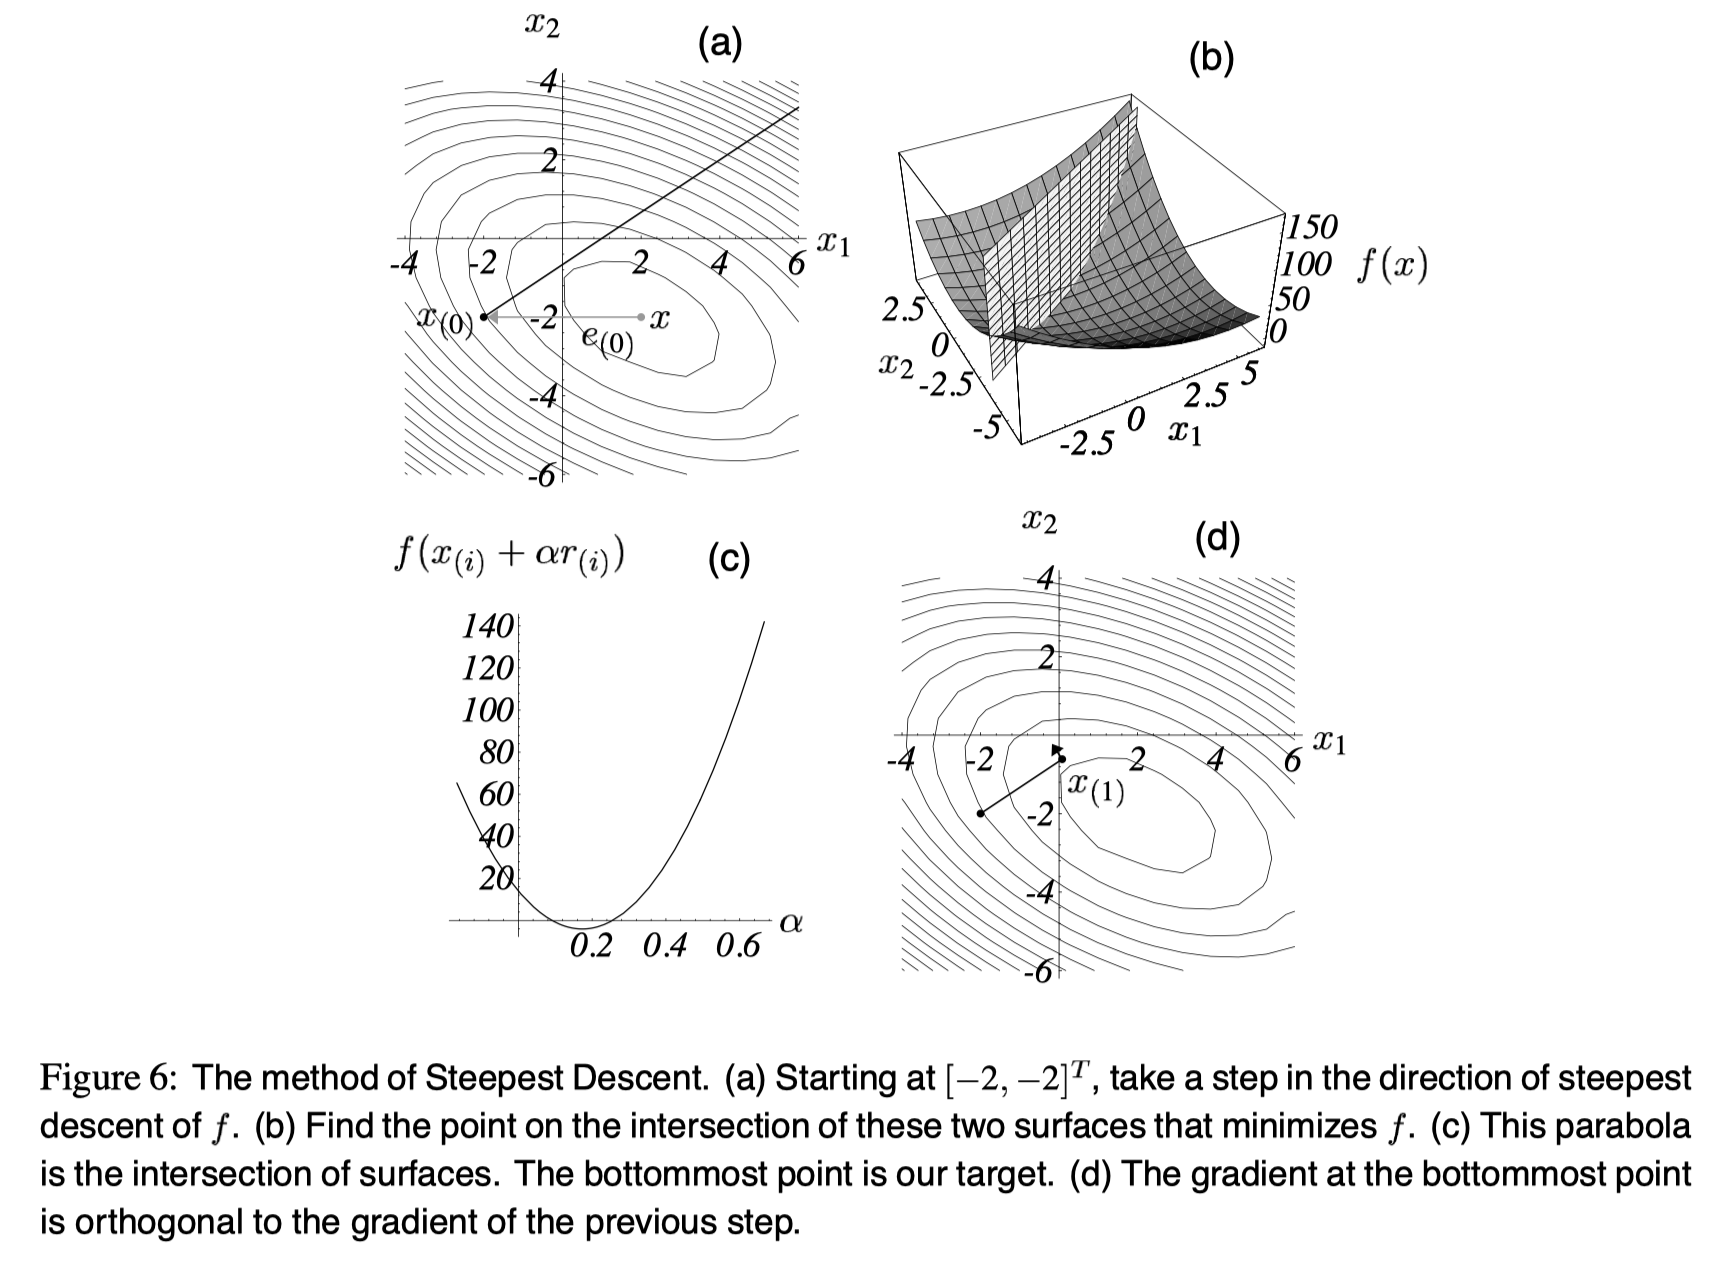
\includegraphics[width=1\textwidth]{fig/CG_Plot_SD_1.png}
\end{figure}

另外,从图7也可以看出来,为什么 $f'(x_1)$ 需要与 $r_0$ 正交。图7的实线方向是 $f'(x_1)$ 的方向(也就是 line search 的方向),该实线上不同的点有不同的梯度方向(实线箭头),对应了 $f$ 的不同的下降速率(虚线箭头),显然当下降速率为 0 时,$f$ 下降的最多,也就是说,此时的梯度与 $f'(x_1)$ 是正交的。
\begin{figure}[H]
    \centering
    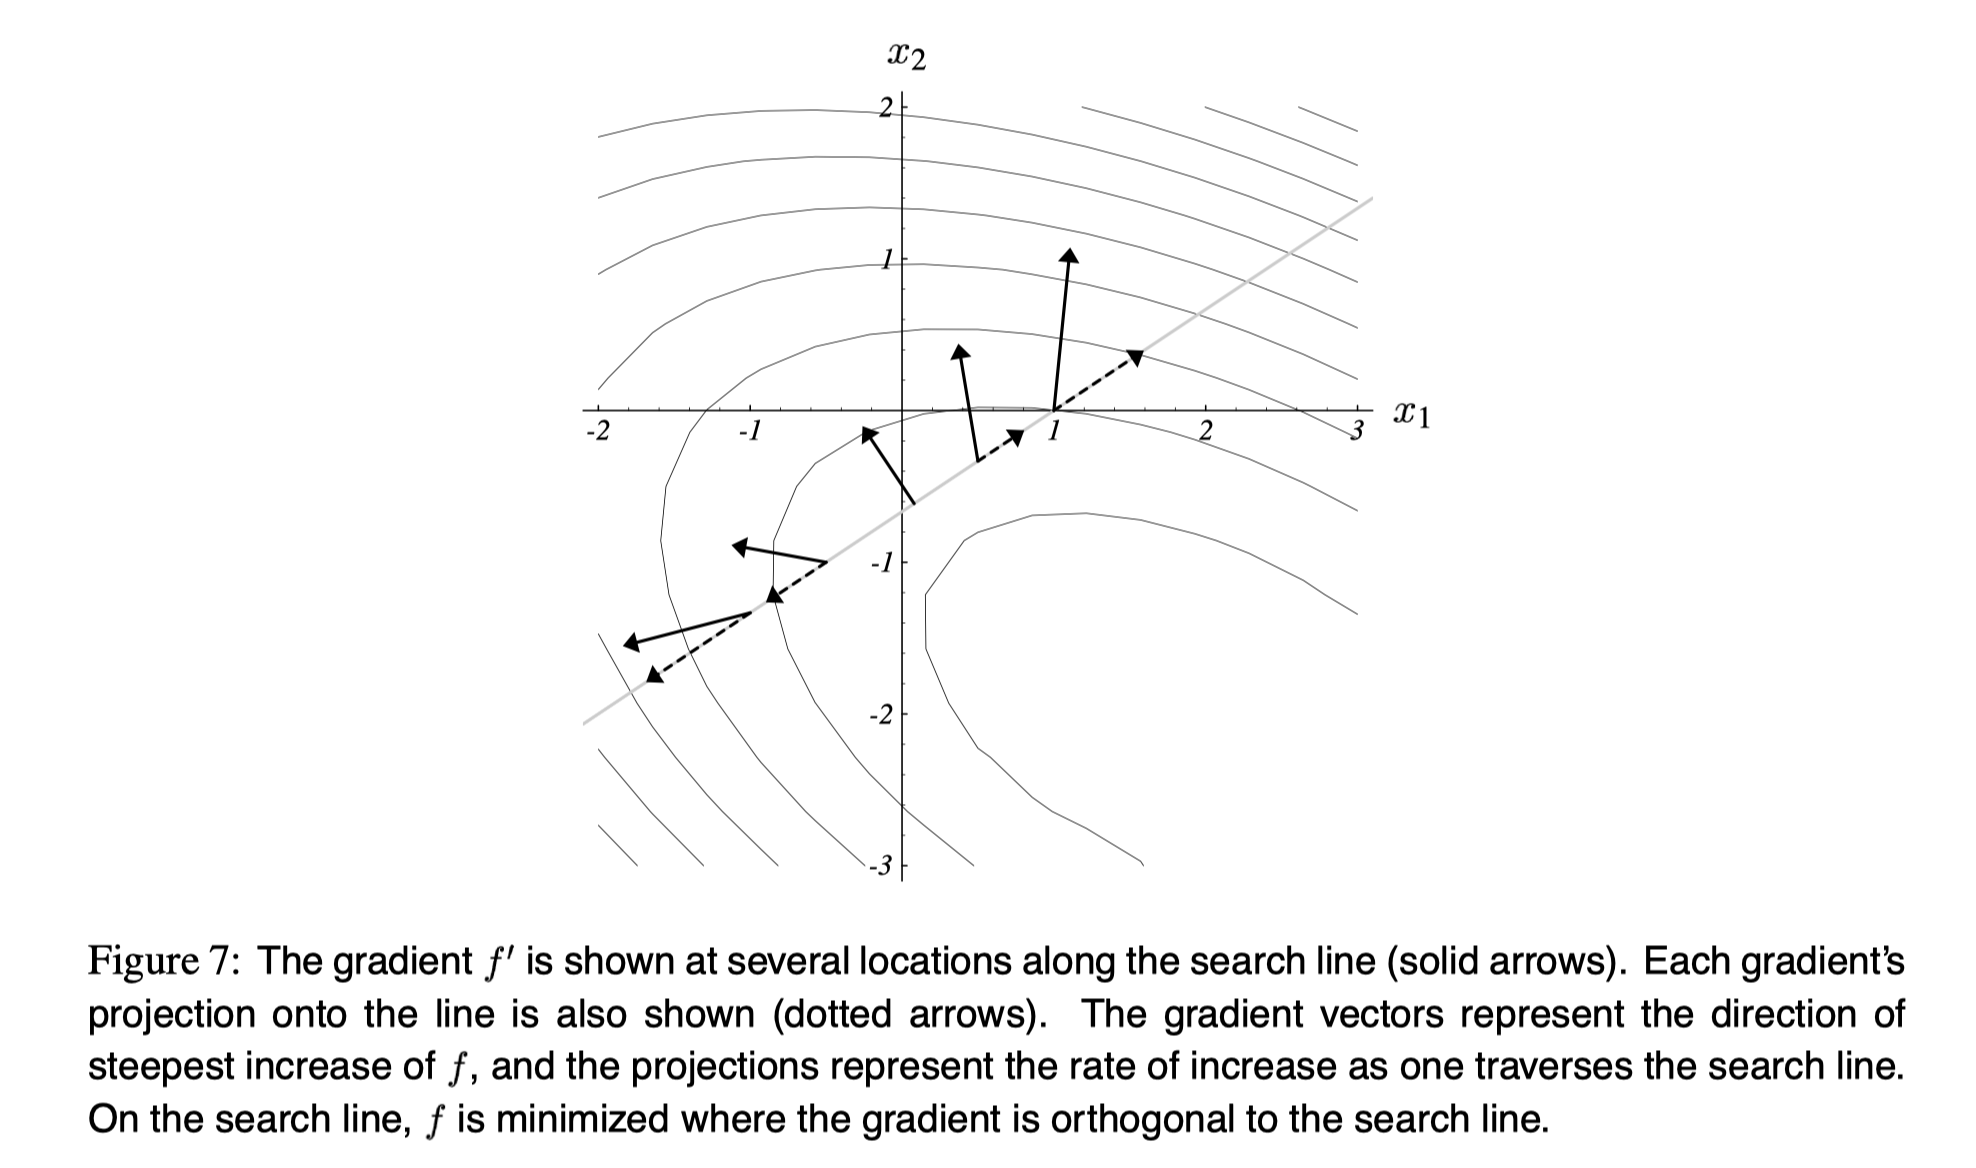
\includegraphics[width=1\textwidth]{fig/CG_Plot_SD_2.png}
\end{figure}

因为有 $f'(x_1) = -r_1$,所以可以如下推导出 $\alpha$:
\begin{align*}
f'(x_1) r_0 &= 0 \Rightarrow \\
r_1^T r_0 &= 0 \Rightarrow \\
(b - Ax_1)^T r_0 &= 0 \\
(b - A(x_0 + \alpha r_0))^T r_0 &= 0 \\
(b - Ax_0)^T r_0 - \alpha (A r_0)^T r_0 &= 0 \\
(b - Ax_0)^T r_0 &=  \alpha (A r_0)^T r_0 \Rightarrow \\
r^T_0 r_0 &= \alpha r^T_0(Ar_0) \Rightarrow \\
\alpha &= \frac{r^T_0 r_0 }{r^T_0 A r_0}
\end{align*}

汇总后,就得到了最速下降法的具体过程:
$$
r_i = b - Ax_i
$$
$$
\alpha_i = \frac{r^T_i r_i }{r^T_i A r_i}
$$
$$
x_{i+1} = x_i + \alpha_i r_i
$$

图8是该过程的具体示例:
\begin{figure}[H]
    \centering
    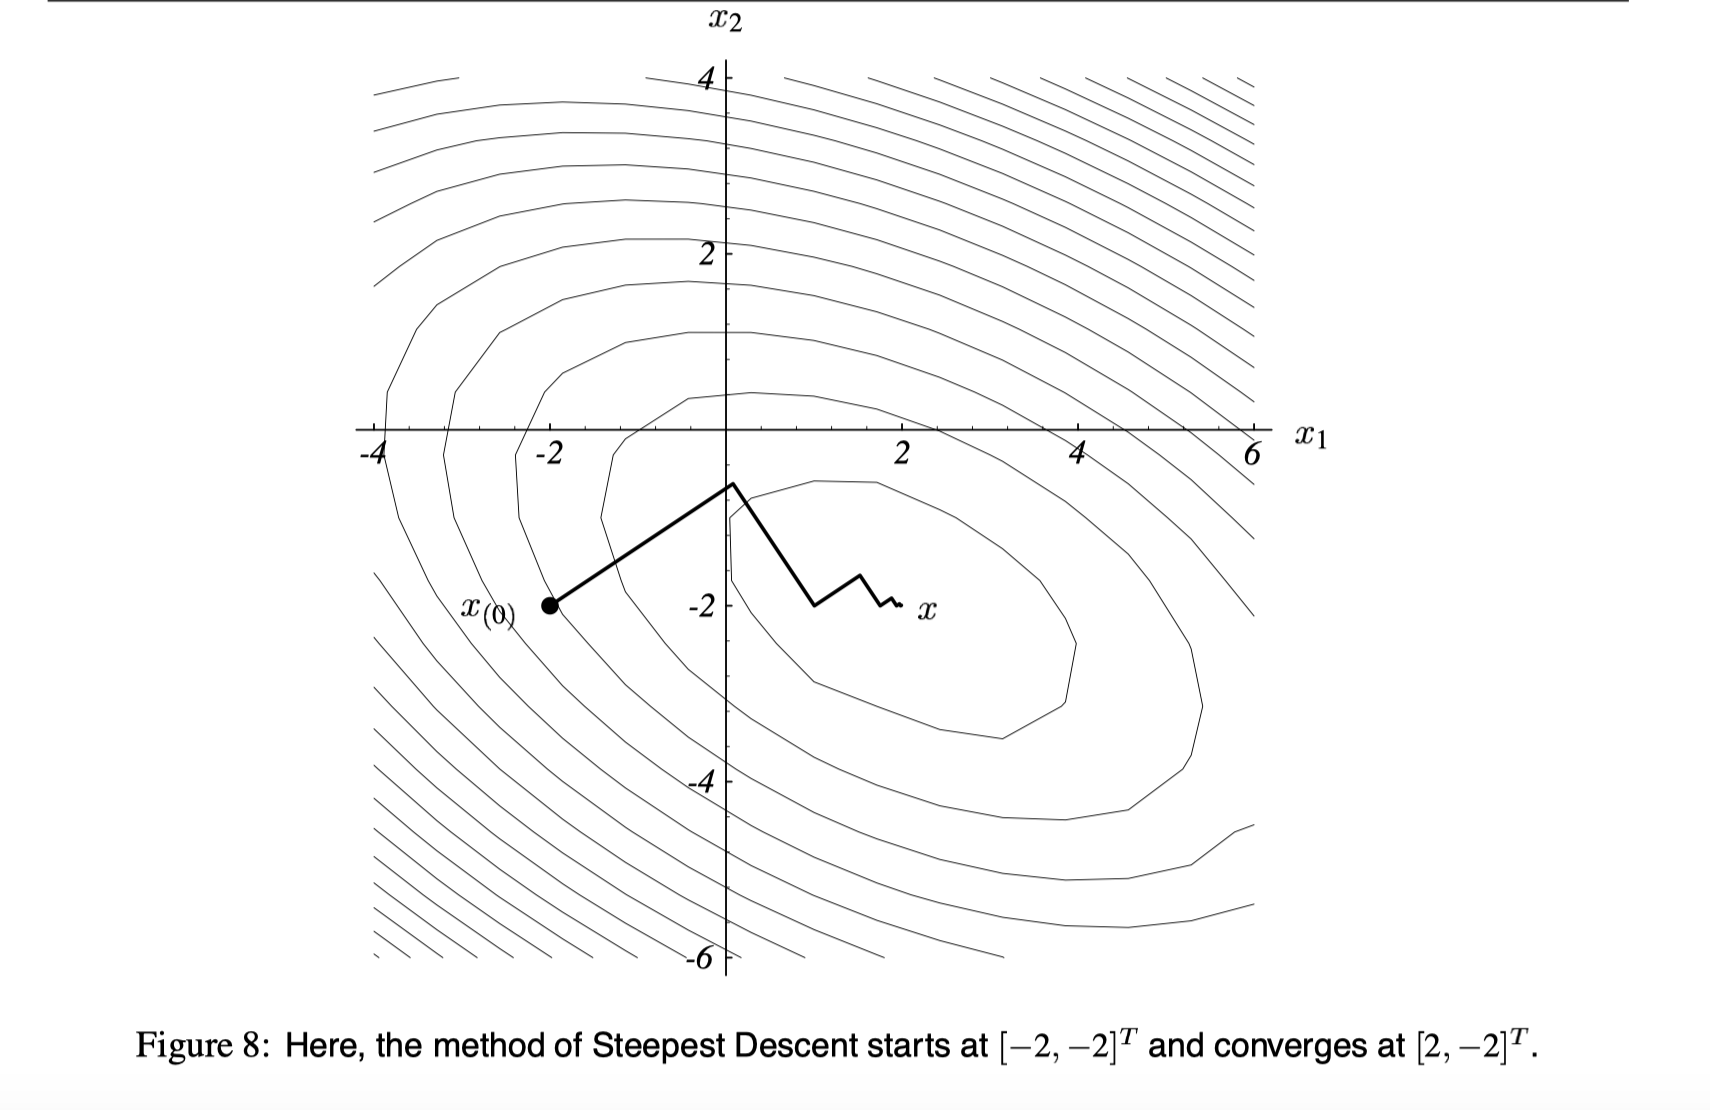
\includegraphics[width=.8\textwidth]{fig/CG_Plot_SD_3.png}
\end{figure}

\section{Jacobi iterations}
\subsection{算法介绍}
使用 Jacobi 迭代法求解 $Ax = b$ 的过程如下:首先将 $A$ 分位两部分:$A = D + E$;其中 $D$ 是 $A$ 的对角元素,其余元素为0;$E$ 是 $A$ 的非对角元素,对角元素为0。然后,按如下步骤求解:
\begin{align*}
Ax &= b \\
(D+E) x &= b \\
Dx &= -Ex + b \\
x &= -D^{-1}Ex + D^{-1}b \\
x &= Bx + z, \qquad B = -D^{-1}E, z = D^{-1}b
\end{align*}

因为 $D$ 是对角线矩阵,所以很容易求逆。同时,观察最后一项:$x = Bx + z$ 可知,该方程的解 $x$ 是其驻点(stationary point),也就是说当 $x_i = x$ 时,有 $x_{i+1} = x$;因此可以按照如下迭代的方法求解 $x$:
$$
x_{i+1} = Bx_i + z
$$

事实上,对 $A$ 进行不同类型的分解,可以得到不同的解法,如 Gauss-Seidel 法,Successive Over-Relaxation(SOR)法等;

\textbf{为了使迭代过程尽快收敛,显然需要 $B$ 有尽量小的谱半径}。

\subsection{收敛性分析}
假定从任意点 $x_0$ 出发,每步迭代都有 $x_{i+1} = Bx_i + z$,将 $x_i$ 分解为 $x$ 和误差 $e_i$ 的和,有:
\begin{align*}
x_{i+1} &= Bx_i + z \\
 	   &= B(x + e_i) + z \\
	   &= Bx + z + Be_i \\
	   &= x + Be_i \\
\therefore e_{i+1} &= Be_i
\end{align*}

所以,如果 $\rho(B) < 1$,那么误差项 $e_i$ 可以收敛至0,也就是说,选择任意初始向量 $x_0$ 都不会影响最终结果。虽然 $x_0$显然会影响迭代步数,但是起决定性因素的还是 $\rho(B)$ 。\textbf{如果 $v_j$ 是$B$ 中具有最大特征值$\lambda_j$ 的特征向量,即 $\rho(B) = \lambda_j$。如果初始误差 $e_0$ 按照 $B$ 的特征向量分解后,包含 $v_j$ 方向的部分,那么这部分收敛至0的速度是最慢的}。

\subsection{Jacobi iterations 算法的缺陷}
一般来说,即使 $A$ 是对称矩阵,$B$ 也未必是对称矩阵;并且,$B$ 可能不存在特征向量;Jacobi iterations 的收敛速度取决于 $rou(B)$,$B$ 又取决于 $A$;然而,即使 $A$ 是正定矩阵,Jacobi 方法也未必能保证收敛。


\subsection{一个具体的例子}
给定矩阵 $A = \begin{bmatrix} 3 & 2 \\ 2 & 6 \end{bmatrix}, b = \begin{bmatrix} 2 \\ -8 \end{bmatrix}$,按照 Jacobi 方法,将 $A$ 进行分解,有:$A = D + E$,其中:
$$
D = \begin{bmatrix} 3 & 0 \\ 0 & 6\end{bmatrix} \qquad E = \begin{bmatrix} 0 & 2 \\ 2 & 0\end{bmatrix}
$$

进而有:
$$
D^{-1} = \begin{bmatrix} 1/3 & 0 \\ 0 & 1/6\end{bmatrix} 
$$
$$
D^{-1} E = \begin{bmatrix} 0 & 2/3 \\ 1/3 & 0\end{bmatrix} \qquad D^{-1} b = \begin{bmatrix} 2/3 \\ -4/3\end{bmatrix} 
$$

所以可以得到如下迭代过程:
\begin{align*}
x_{i+1} &= -D^{-1}Ex + D^{-1}b \\
          &= \begin{bmatrix} 0 & -2/3 \\ -1/3 & 0\end{bmatrix}x_i + \begin{bmatrix} 2/3 \\ -4/3\end{bmatrix}
\end{align*}

$B$ 的特征向量分别为:$v_1 = [\sqrt{2}, 1]^T, v_2 = [-\sqrt{2}, 1]^T$,对应的特征向量分别为:$\lambda_1 = -\sqrt{2}/3, \lambda_2 = \sqrt{2}/3$。从下面的图13(a)可以看出,$B$ 的特征向量与 $A$ 并不重合;图13(b) 表明了 Jacobi 方法的收敛过程,中间每一步的特征向量的变化在图13(c)(d)(e)(f) 中有展示。
\begin{figure}[H]
    \centering
    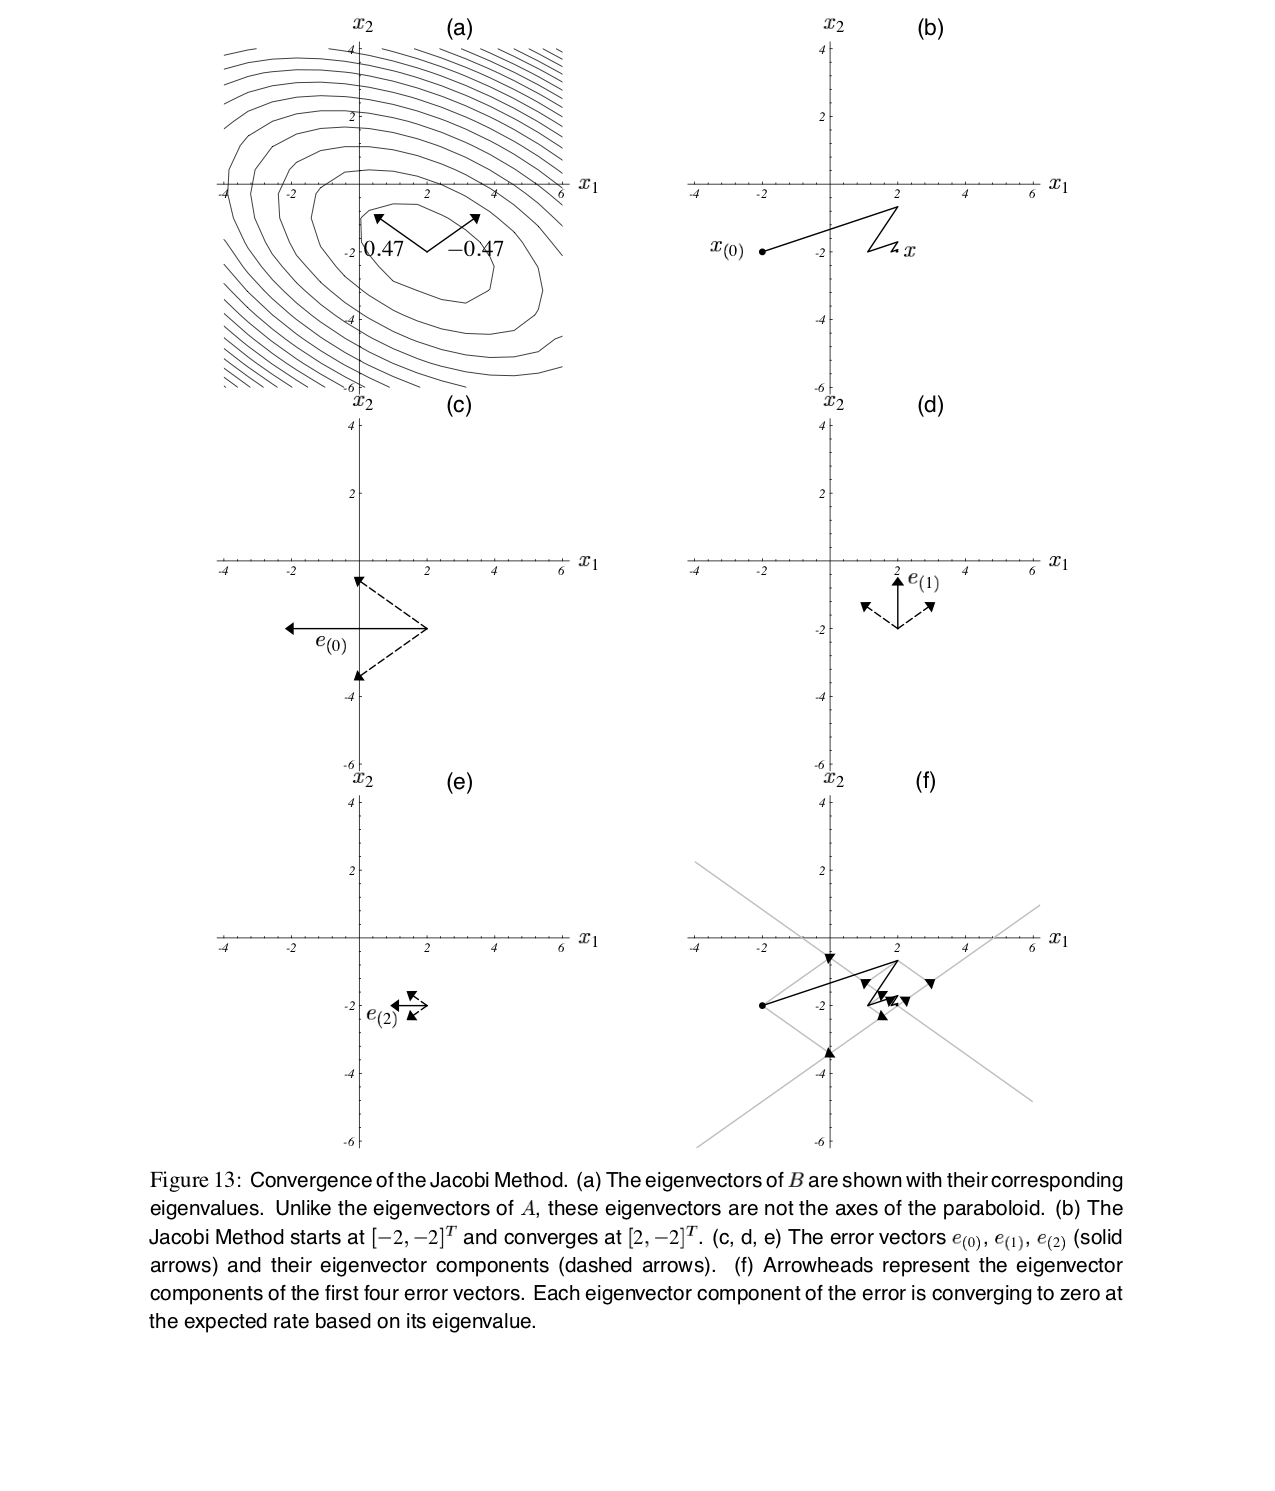
\includegraphics[width=1\textwidth]{fig/CG_Convergence_Jacobi_1.png}
\end{figure}

\section{最速下降法的收敛性分析}
\subsection{误差与特征向量同向的情况}
首先考虑下误差 $e_i$ 刚好是 $A$ 的特征向量的情况,对应的特征值为 $\lambda_e$。那么,余量 $r_i = -Ae_i = -\lambda_ee_i$ 同样也是 $A$ 的特征向量。根据之前推导的 $x_{i+1} = x_i + \alpha_i r_i$,且$e_i = x_i - x$,有:
\begin{align*}
e_{i+1} &= x_{i+1} - x \\
	   &= x_i + \alpha_ir_i - x \\
	   &= x_i - x + \alpha_ir_i \\
	   &= e_i + \frac{r^T_ir_i}{r^T_iAr_i}r_i  \\
	   &= e_i + \frac{r^T_ir_i}{\lambda_er^T_ir_i}(-\lambda_ee_i) \\
	   &= 0
\end{align*}

图14是这种类型的示例,因为 $x_i$ 位于椭圆的轴上,所以余量 $r_i$ 指向了椭圆的中心,选择 $\alpha_i = \lambda^{-1}_e$,可以立刻收敛。
\begin{figure}[H]
    \centering
    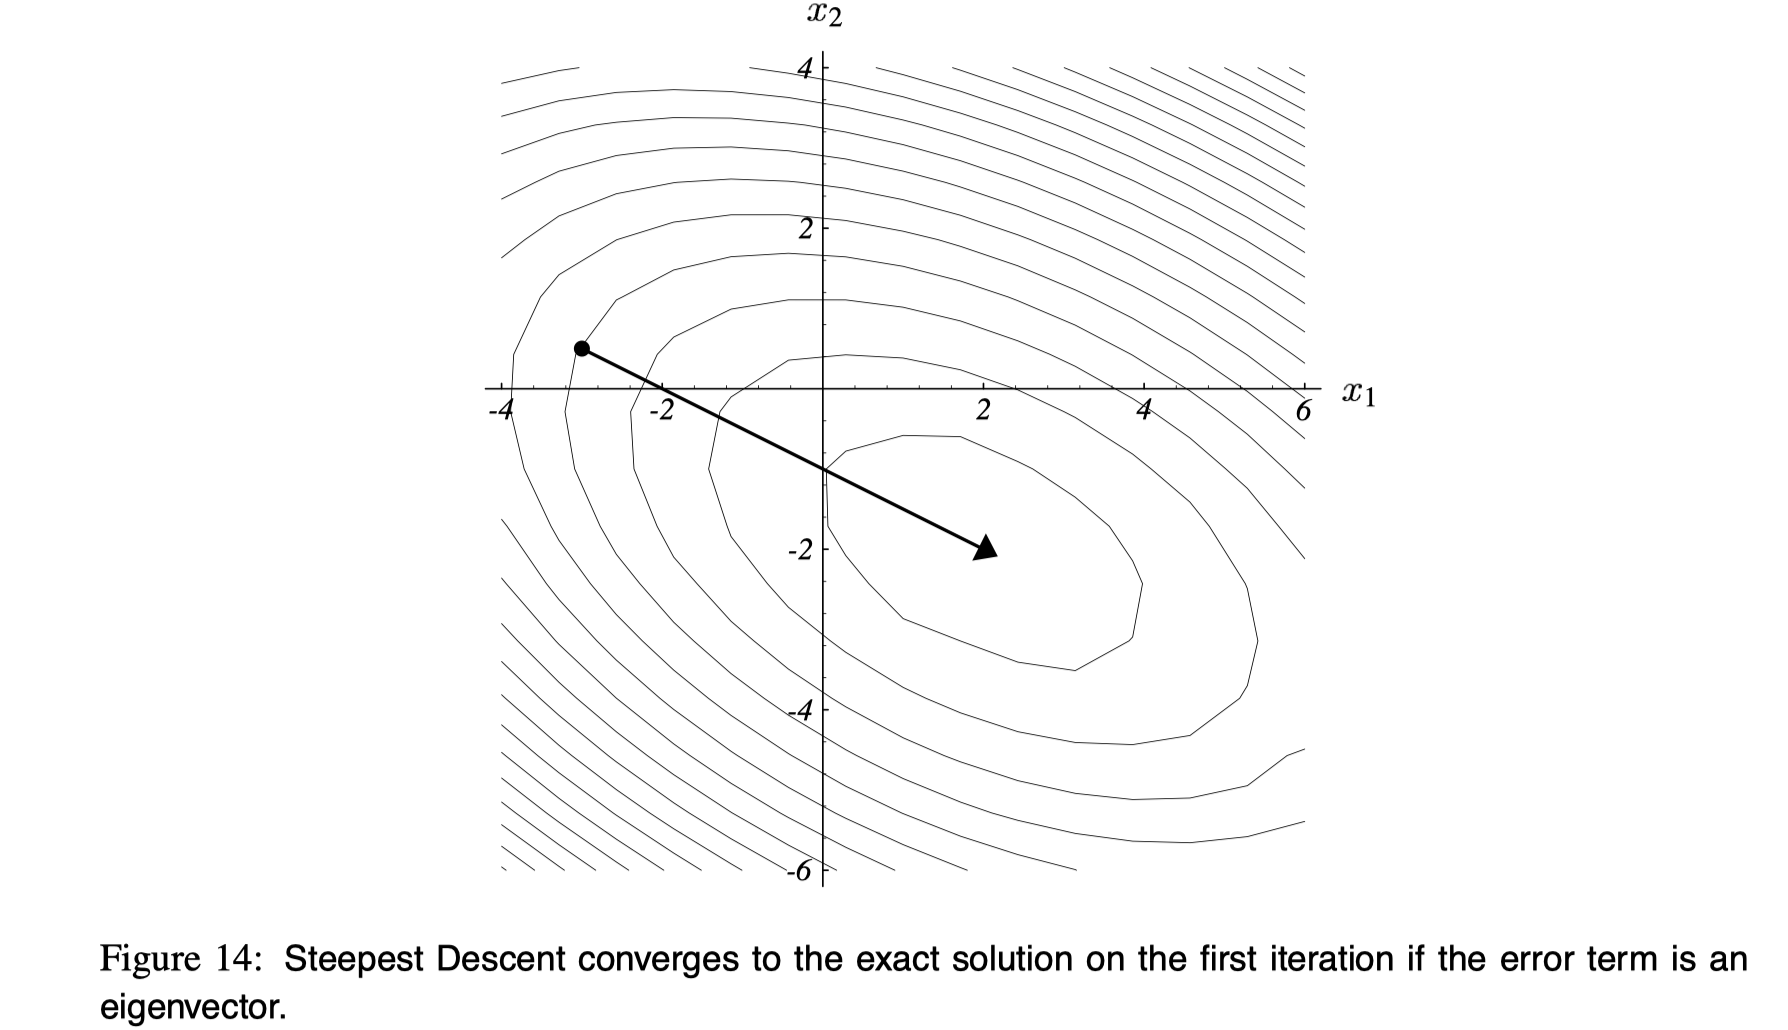
\includegraphics[width=1\textwidth]{fig/CG_Convergence_SD_1.png}
\end{figure}

\subsection{特征值相同的情况}
对于一般情况下的 $e_i$,将 $e_i$ 表示为特征向量的线性组合,因为特征向量可以任意进行比例变换,为了方便讨论,令特征向量的长度均为单位长度。因为当 $A$ 是对称矩阵时,其特征向量都是正交的,那么有:
$$
v_j^Tv_k = \begin{cases} 1, \qquad j = k \\ 0, \qquad j \neq k \end{cases}
$$

将 $e_i$ 表示为特征向量的线性组合形式如下:
$$
e_i = \sum_{j=1}^n \xi_j v_j
$$

因此,有:
\begin{align*}
&r_i = -A e_i = -\sum_j\xi_j\lambda_jv_j \\
&||e_i||^2 = e^T_ie_i = \sum_j\xi_j^2 \\
&||r_i||^2 = r^T_ir_i = \sum_j\xi_j^2\lambda_j^2 \\
&e^T_iAe_i = (\sum_j\xi_jv_j^T)(\sum_j\xi_j\lambda_jv_j) = \sum_j \xi_j^2\lambda_j \\
&r^T_iAr_i = \sum_j\xi_j^2\lambda_j^3 \\
\end{align*}

从第1个式子可以看出来,$r_i$ 也可以表示为特征向量的线性组合,并且每个分量的长度为 $-\xi_j\lambda_j$。

那么,根据 $x_{i+1} = x_i + \alpha r_i$,有:
\begin{align*}
e_{i+1} &= e_i + \frac{r^T_ir_i}{r^T_iAr_i}r_i \\
	   &= e_i + \frac{\sum_j\xi^2_j\lambda^2_j}{\sum_j\xi^2_j\lambda^3_j}r_i
\end{align*}

如果所有的特征向量都有相同的特征值 $\lambda$,即 $\lambda_j = \lambda, j = 1, 2, \cdots, n$,因为 $e_i = \sum_{j=1}^n \xi_j v_j$,且 $r_i =  -\sum_j\xi_j\lambda_jv_j $,那么就有:$r_i =  -\lambda \sum_j\xi_jv_j = -\lambda e_i$

所以,有:
\begin{align*}
e_{i+1} &= e_i + \frac{\lambda^2\sum_j\xi^2_j}{\lambda^3\sum_j\xi^2_j}(-\lambda e_i) \\
&= 0
\end{align*}

如图15所示,因为所有的特征值都相同,所以原来的椭圆变成了圆形。因此,无论从任何点出发,余量都必然指向圆心。这时,只要选择 $\alpha_i = \lambda^{-1}$,一步就可以收敛。
\begin{figure}[H]
    \centering
    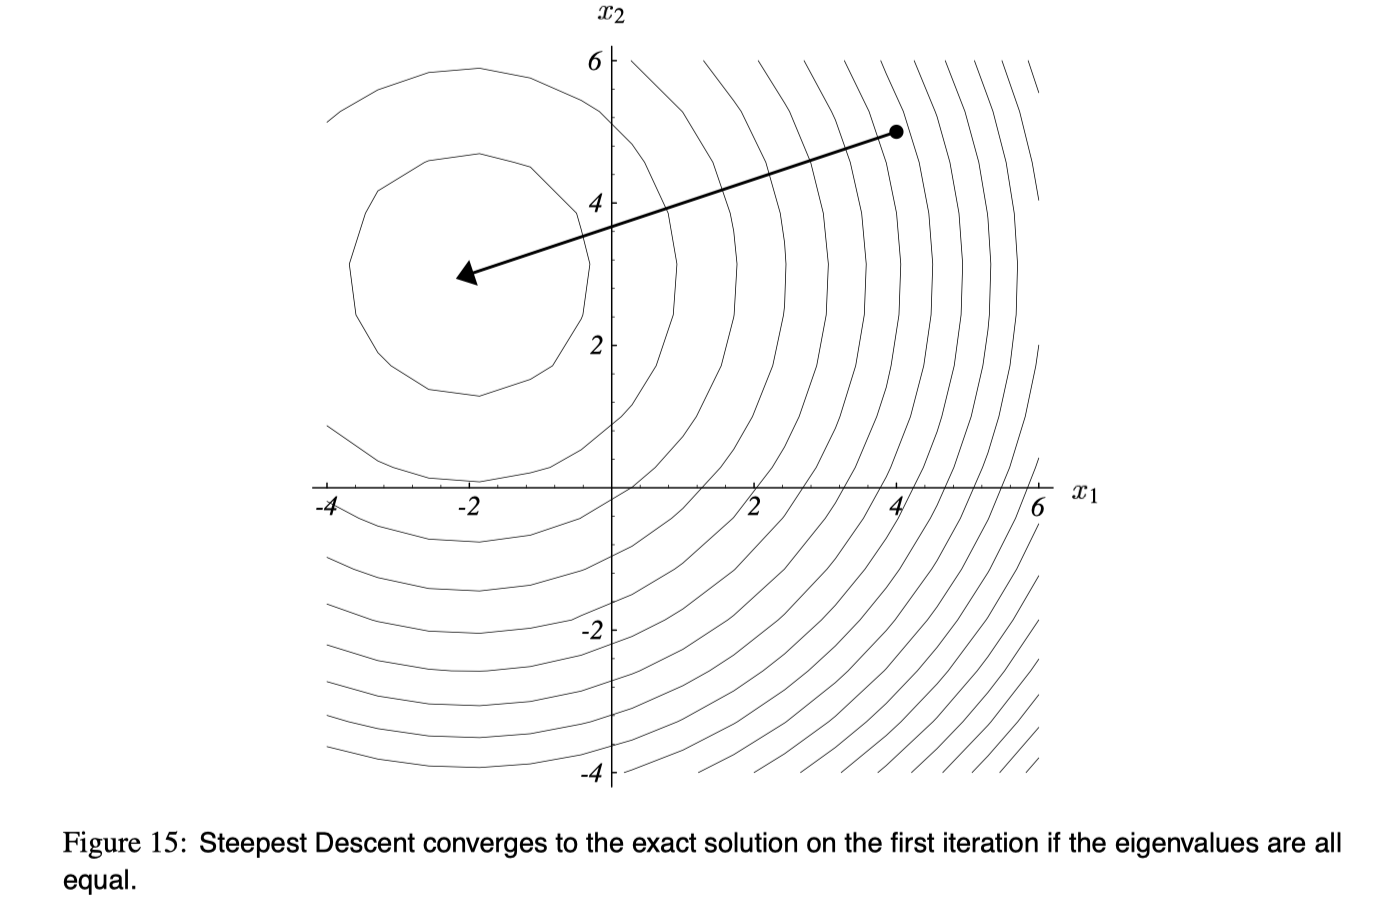
\includegraphics[width=1\textwidth]{fig/CG_Convergence_SD_2.png}
\end{figure}

如果存在若干个不相等的非零特征值,那么就没有合适的 $\alpha_i$ 能够同时消除所有的特征向量分量。这时 $\alpha_i$ 的选择就变成了$\lambda_j^{-1}$的加权平均,权重 $\xi^2_j$确保 $e_i$ 的“长分量”会被优先处理;因此,在每一步的迭代中,$e_i$ 的“短分量”甚至有可能会变大(当然不会一直边长)。所以,最速下降法和共轭梯度法通常被称为 roughers;而 Jacobi 法被称为 smoother,因为在每次迭代中,所有的特征向量分量都会减少。

\subsection{一般情况}
为了分析一般情况下 SD 的收敛情况,定义 energy norm 如下:
$$
||e||_A = (e^TAe)^{1/2}
$$

根据之前的推导,$f(p) = f(x) + \frac{1}{2}(p-x)^TA(p-x)$,我们知道最小化 $||e_i||_A$ 等价于最小化 $f(x_i)$。因此,有:
\begin{align*}
||e_{i+1}||^2_A &= e^T_{i+1}Ae_{i+1} \\
	&= (e^T_i + \alpha_i r^T_i)A(e_i + \alpha_i r_i) \\
	&= e^T_iAe_i + 2\alpha_ir^T_iAe_i + \alpha^2_ir^T_iAr_i \\
	&= ||e_i||^2_A + 2\frac{r^T_ir_i}{r^T_iAr_i}\Big(-r^T_ir_i\Big) + \Big(\frac{r^T_ir_i}{r^T_iAr_i}\Big)^2r^T_iAr_i  \qquad (r_i = -Ae_i)\\
	&= ||e_i||^2_A - \frac{(r^T_ir_i)^2}{r^T_iAr_i} \\
	&=  ||e_i||^2_A - \frac{||e_i||^2_A}{ ||e_i||^2_A}\cdot\frac{(r^T_ir_i)^2}{r^T_iAr_i} \\
	&=  ||e_i||^2_A - \frac{||e_i||^2_A}{e^T_iAe_i}\cdot\frac{(r^T_ir_i)^2}{r^T_iAr_i} \\
	&= ||e_i||^2_A \Bigg(1 - \frac{(r^T_ir_i)^2}{(r^T_iAr_i)(e^T_iAe_i)}\Bigg) \\
	&= ||e_i||^2_A \Bigg(1 - \frac{(\sum_j\xi_j^2\lambda_j^2)^2}{(\sum_j\xi_j^2\lambda_j^3)(\sum_j\xi_j^2\lambda_j)}\Bigg) \\
	&= ||e_i||^2_A\omega^2, \qquad \omega^2 = 1 - \frac{(\sum_j\xi_j^2\lambda_j^2)^2}{(\sum_j\xi_j^2\lambda_j^3)(\sum_j\xi_j^2\lambda_j)}
\end{align*}

接下来,需要分析 $\omega^2$ 的上界。为了分析权重和特征值对收敛性的影响,以 $n=2$ 为例。假定 $\lambda_1 \ge \lambda_2$,$A$ 的\textbf{谱条件数(spectral condition number)}定义为:
$\kappa = \lambda_1 / \lambda_2 \ge 1$,$e_i$的斜率定义为 $\mu = \xi_2 / \xi_1$,因此有:
\begin{align*}
\omega^2 &= 1 - \frac{(\xi_1^2\lambda_1^2 + \xi_2^2\lambda_2^2)^2}{(\xi_1^2\lambda_1 + \xi_2^2\lambda_2)(\xi_1^2\lambda_1^3 + \xi_2^2\lambda_2^3)} \\
	&= 1 - \frac{(\kappa^2 + \mu^2)^2}{(\kappa + \mu^2)(\kappa^3 + \mu^2)}
\end{align*}

$\omega$ 决定了 SD 算法的收敛速度,$\omega$ 和 $\kappa, \mu$ 的关系如下图所示:
\begin{figure}[H]
    \centering
    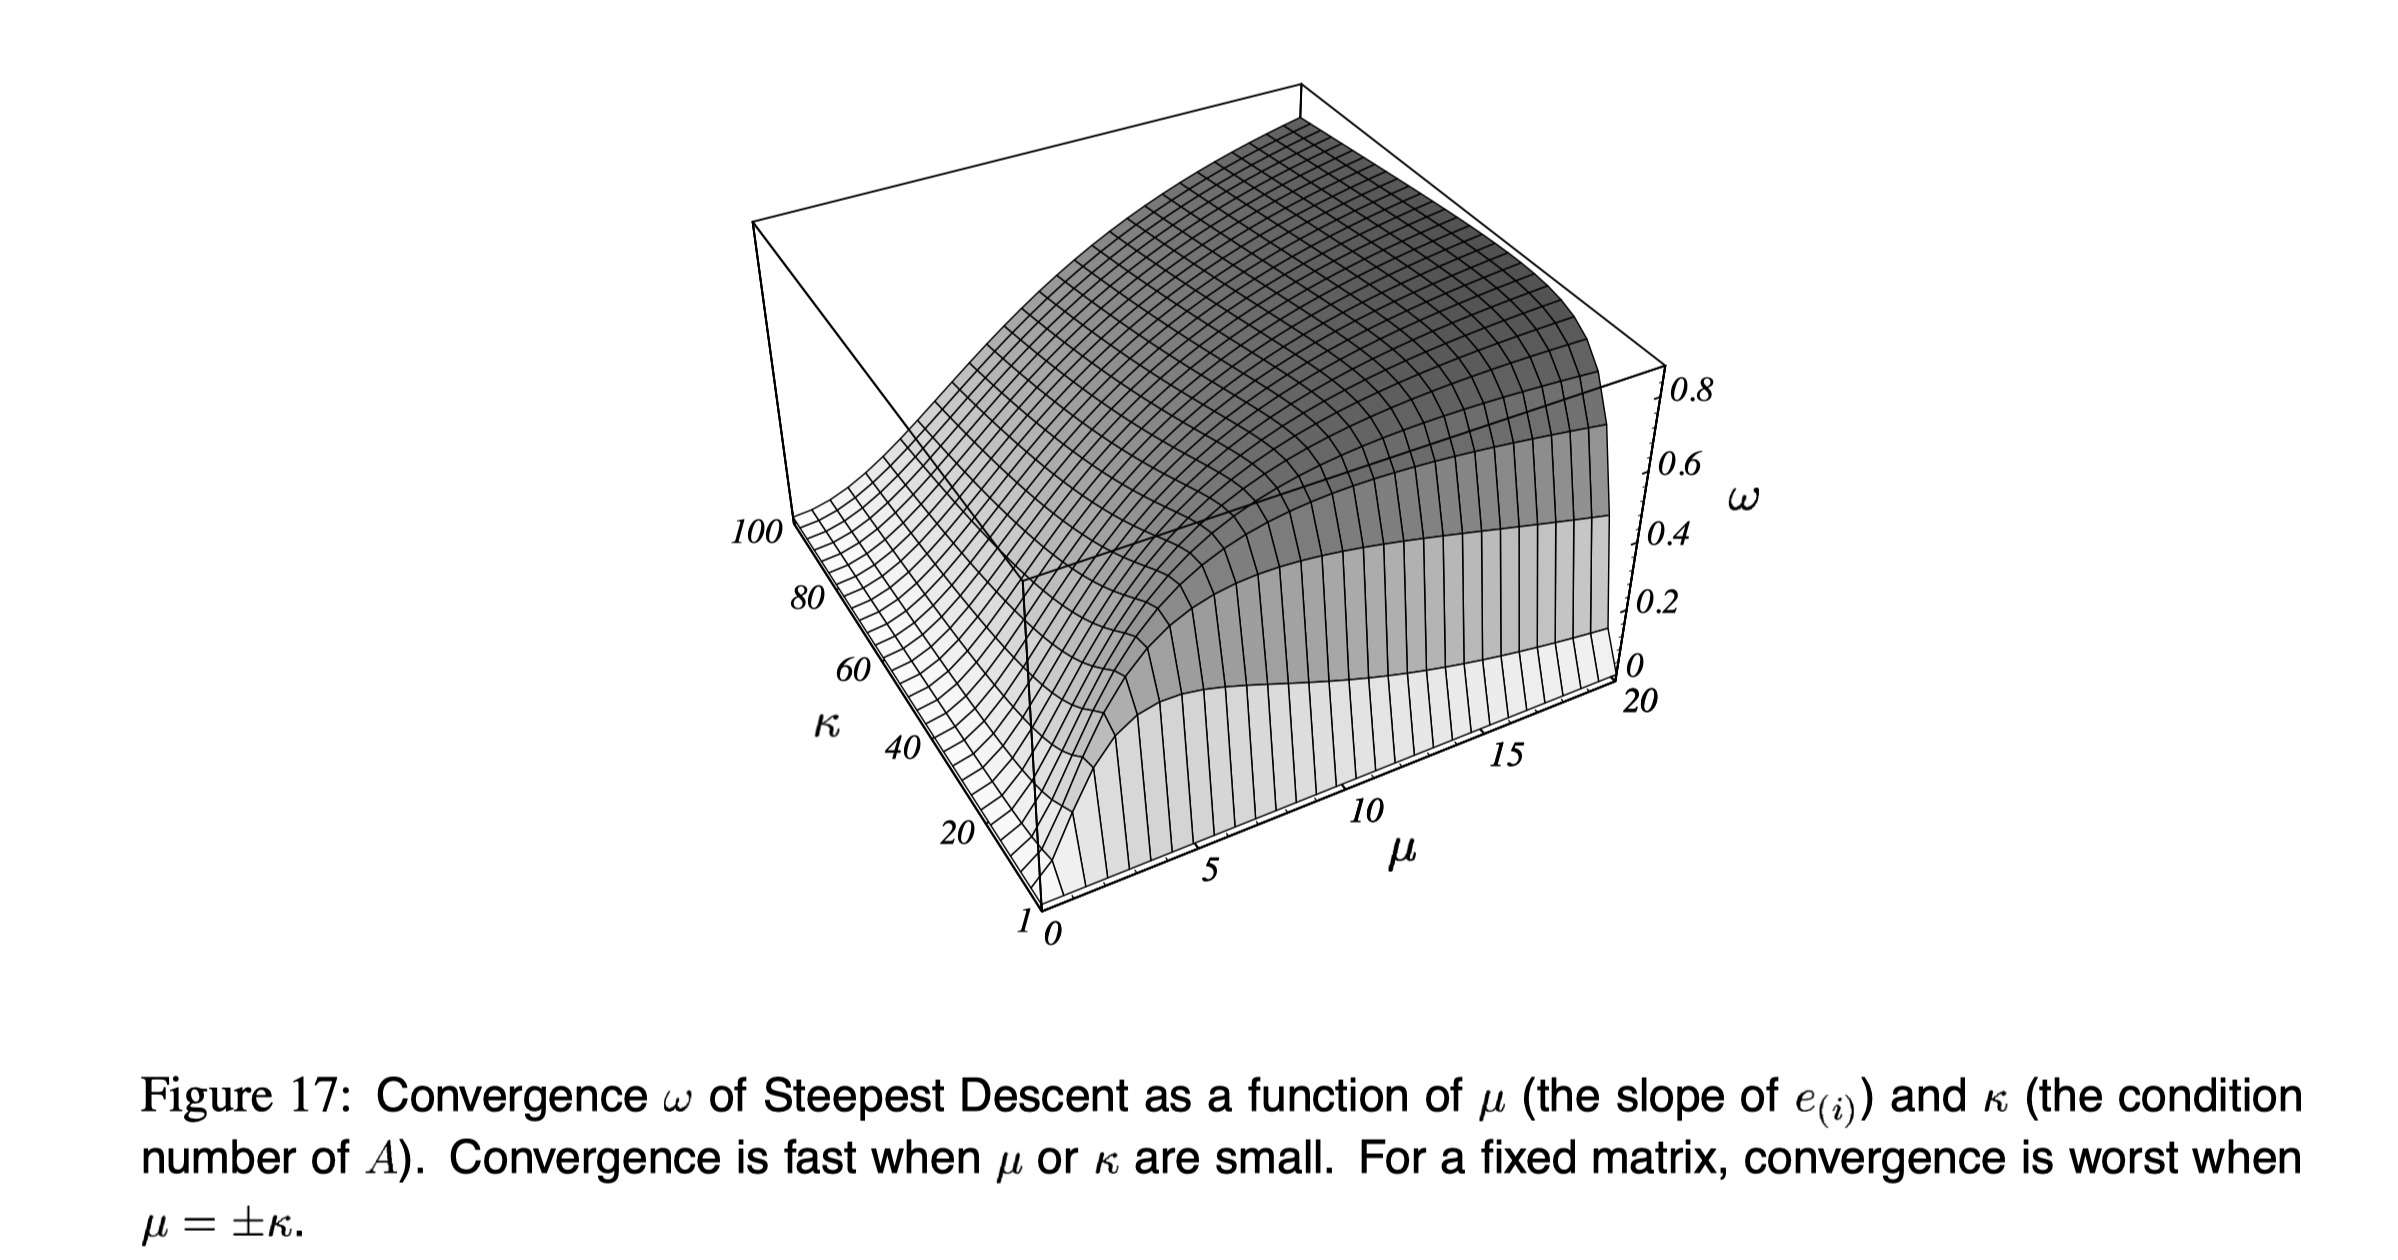
\includegraphics[width=1\textwidth]{fig/CG_Convergence_SD_3.png}
\end{figure}

分如下情况讨论 $\omega$ 的收敛性的影响:
\begin{itemize}
\setlength{\itemsep}{0pt}
\setlength{\parsep}{0pt}
\setlength{\parskip}{0pt}
    \item 如果 $e_0$ 与特征向量同向,那么 $\xi_1 = 0 \ or \ \xi_2 = 0$,斜率 $\mu = 0 \ or \ \mu = \infty$,因此 $\omega = 0$,所以会立刻收敛;
    \item 如果特征值都相等,那么 $\kappa = 1$,因此 $\omega = 0$,所以会立刻收敛;
    \item 从图17中的四个角来讨论下更一般的情况:
    \begin{itemize}
	\setlength{\itemsep}{0pt}
	\setlength{\parsep}{0pt}
	\setlength{\parskip}{0pt}
   	 \item 当条件数很大($\kappa$ 很大)时,如果初始点选择的好,那么 SD 能快速收敛(图18 (a),$\kappa$ 很大,$\mu$ 很小);但是一般情况下,收敛的会比较慢(图18 (b),$\kappa$ 很大,$\mu$ 很大);
	 \item 当条件数很小($\kappa$ 很小)时,二次型近似为圆形,所以无论初始点在哪里,收敛的都比较快(图18 (c),$\kappa$ 很小,$\mu$ 很小;图18 (d),$\kappa$ 很小,$\mu$ 很大);
\end{itemize}
\end{itemize}
\begin{figure}[H]
    \centering
    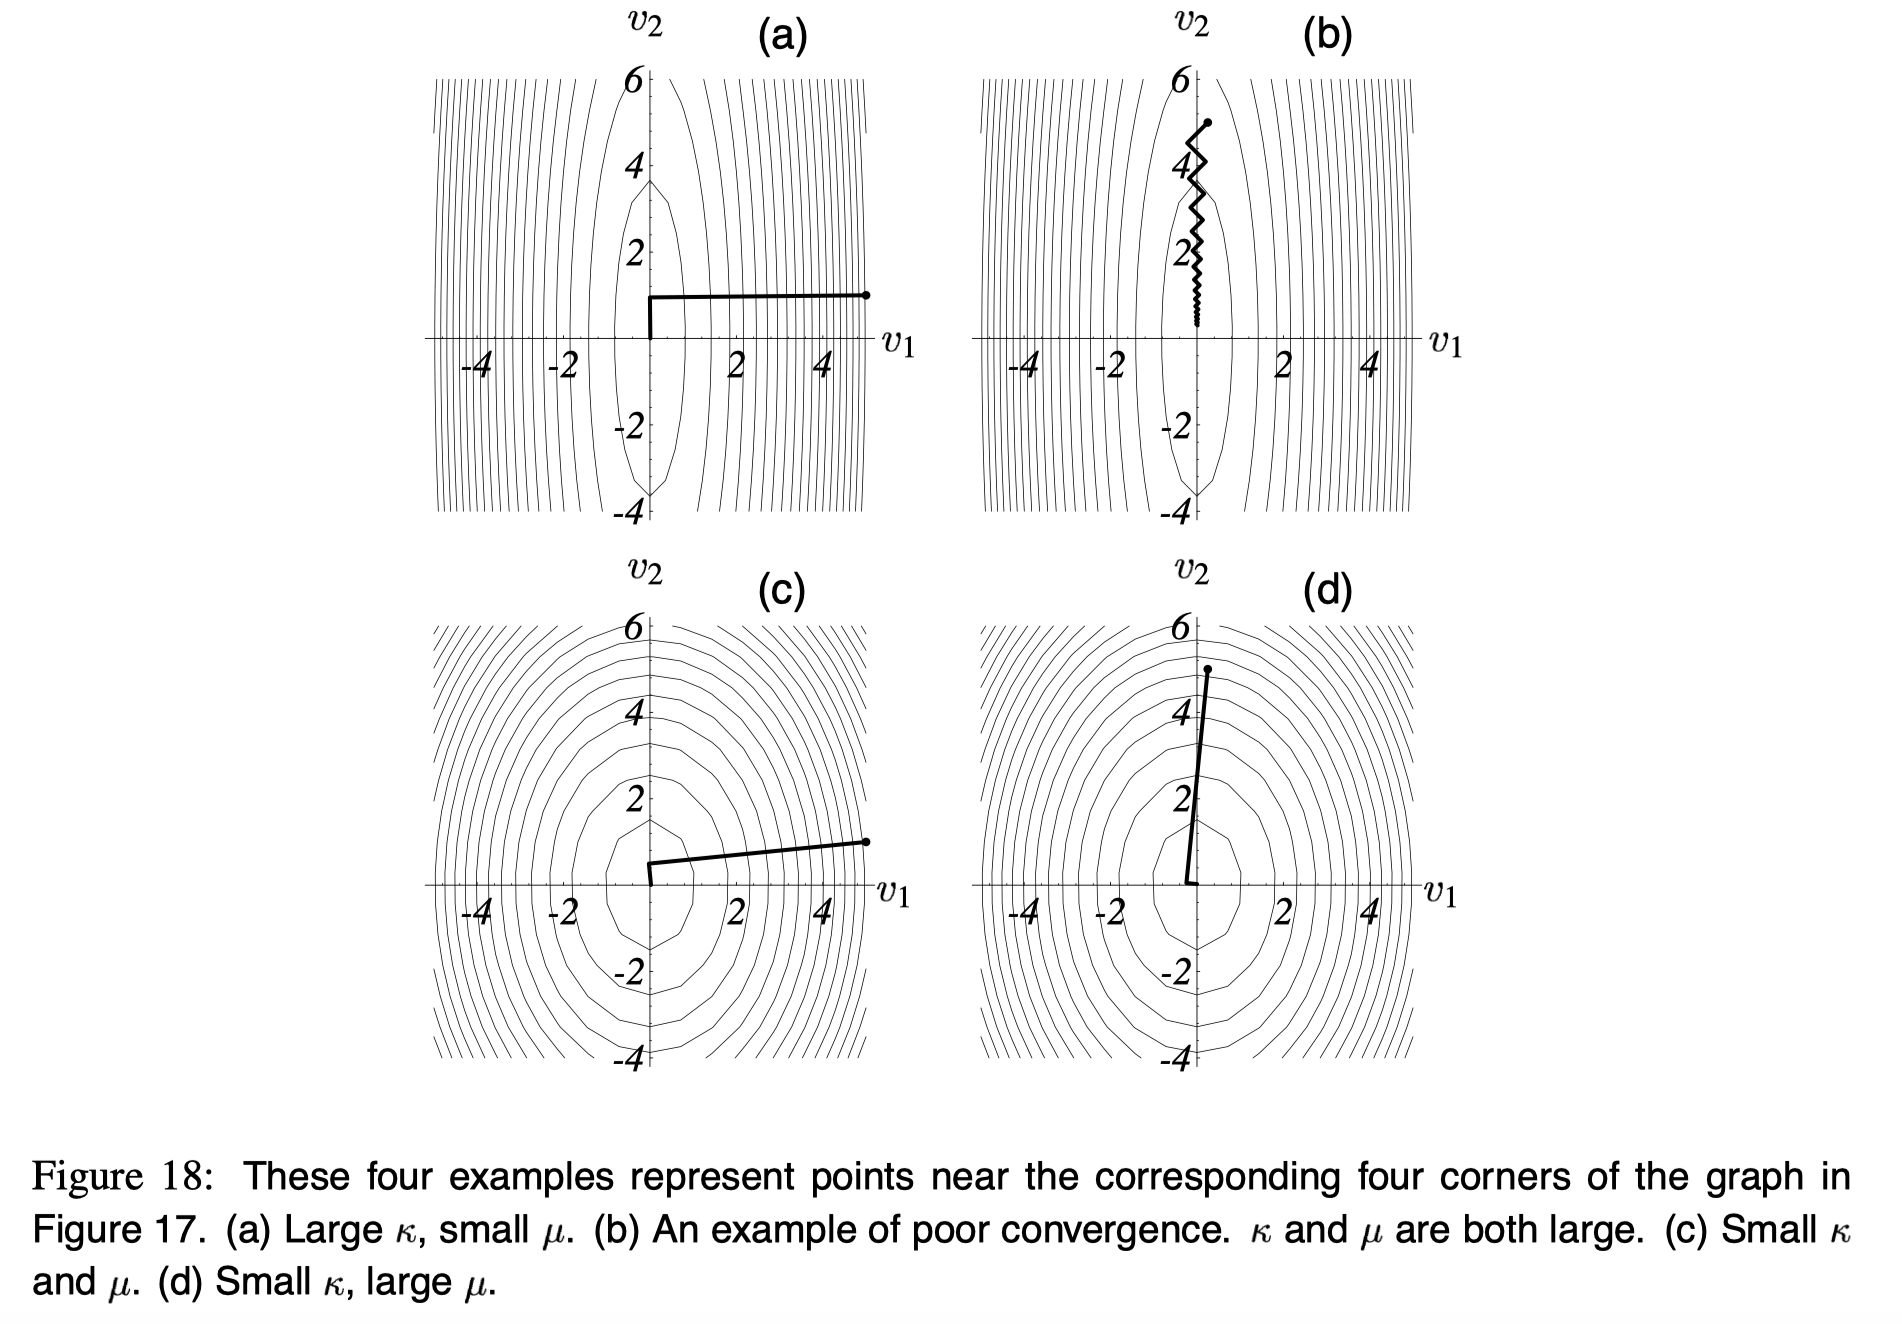
\includegraphics[width=1\textwidth]{fig/CG_Convergence_SD_4.png}
\end{figure}

根据 $\omega$ 的表达式可知,当 $\mu = \pm \kappa$ 时,$\omega$ 取得最大值(从图17中能明显看到一条“山脊”);图19 给出了初始点位于最坏情况下的收敛情况,这些初始点位于 $\xi_2/\xi_1 = \pm \kappa$ 的直线上。当 $\mu^2 = \kappa^2$ 时可以确定 $\omega$ 的上界为
\begin{align*}
\omega^2 &\le 1 - \frac{4\kappa^4}{\kappa^5 + 2\kappa^4 + \kappa^3} \\
	&= \frac{\kappa^5 - 2\kappa^4 + \kappa^3}{\kappa^5 + 2\kappa^4 + \kappa^3}  \\
	&= \frac{(\kappa - 1)^2}{(\kappa + 1)^2} \\
\omega &\le \frac{\kappa - 1}{\kappa + 1}
\end{align*}

图20 给出了 $\omega$ 和 $\kappa$ 的关系;矩阵 $A$ 越病态(ill-conditioned),对应越大的条件数 $\kappa$,SD 算法收敛的越慢;后文可以证明当 $n > 2$ 时,如果该条件数仍定义为对称、正定矩阵的最大和最小特征值的商,即 $\kappa = \lambda_{\max}/ \lambda_{\min}$ ,那么该不等式仍然成立。此时, SD 算法的收敛情况为:
$$
||e_i||_A \le \Big(\frac{\kappa - 1}{\kappa + 1}\Big)^i ||e_0||_A
$$

并且有:
\begin{align*}
\frac{f(x_i) - f(x)}{f(x_0)-f(x)} &= \frac{\frac{1}{2}e^T_iAe_i}{\frac{1}{2}e^T_0Ae_0} \\
&\le \Big(\frac{\kappa - 1}{\kappa + 1}\Big)^{2i}
\end{align*}

\begin{figure}[H]
    \centering
    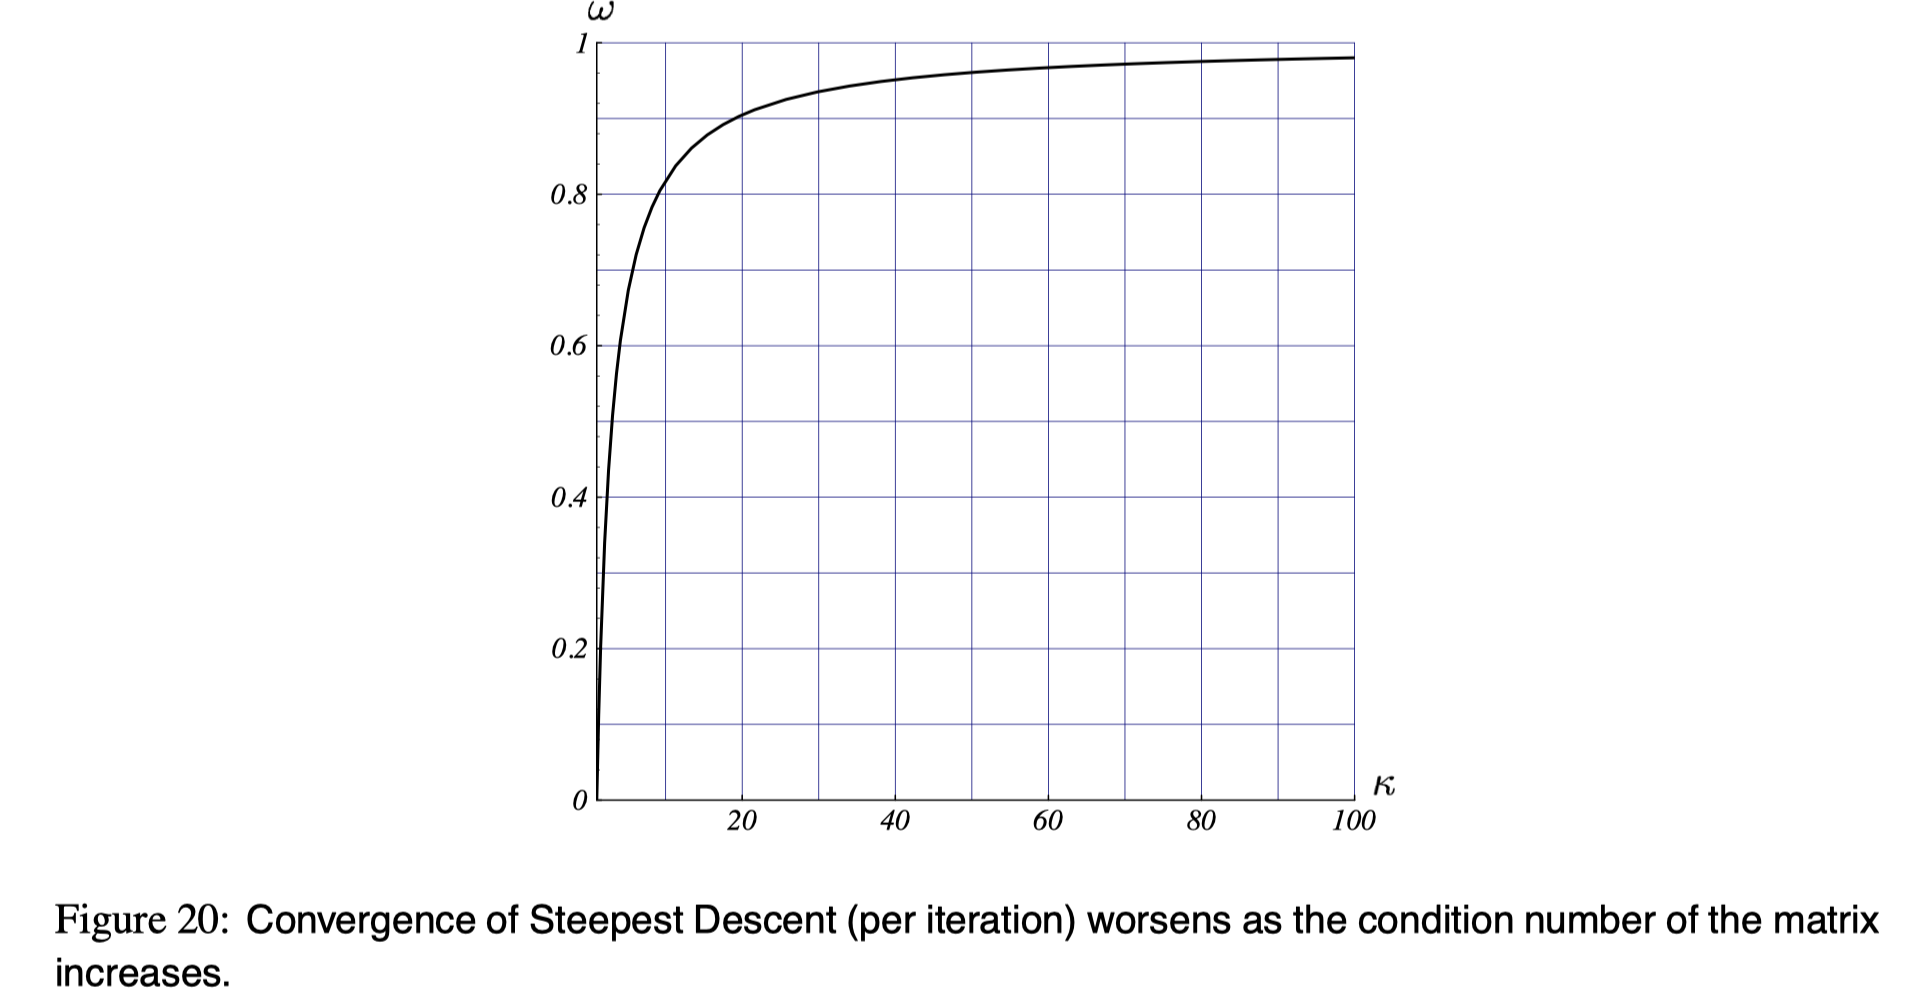
\includegraphics[width=1\textwidth]{fig/CG_Convergence_SD_5.png}
\end{figure}

\section{共轭方向法(The Method of Conjugate Directions)}
\subsection{共轭性(Conjugacy)}
从图8中可以看出, SD 算法在早期的梯度方向是相同的;一个直观的加速收敛的思路是,选择一系列互相正交的方向:$d_0, d_1, \cdots, d_{n-1}$,每一步都走到恰好合适的位置(和 $x$ 对齐),这样经过 $n$ 步后,就收敛到最佳位置了;如图21所示,使用坐标轴的方向作为搜索的方向,第一步沿着正确的 $x_1$轴方向,第二步即收敛了;注意,$e_1$和 $d_0$ 是正交的;也就是说,详细的迭代过程为:
$$
x_{i+1} = x_i + \alpha_i d_i
$$

\begin{figure}[H]
    \centering
    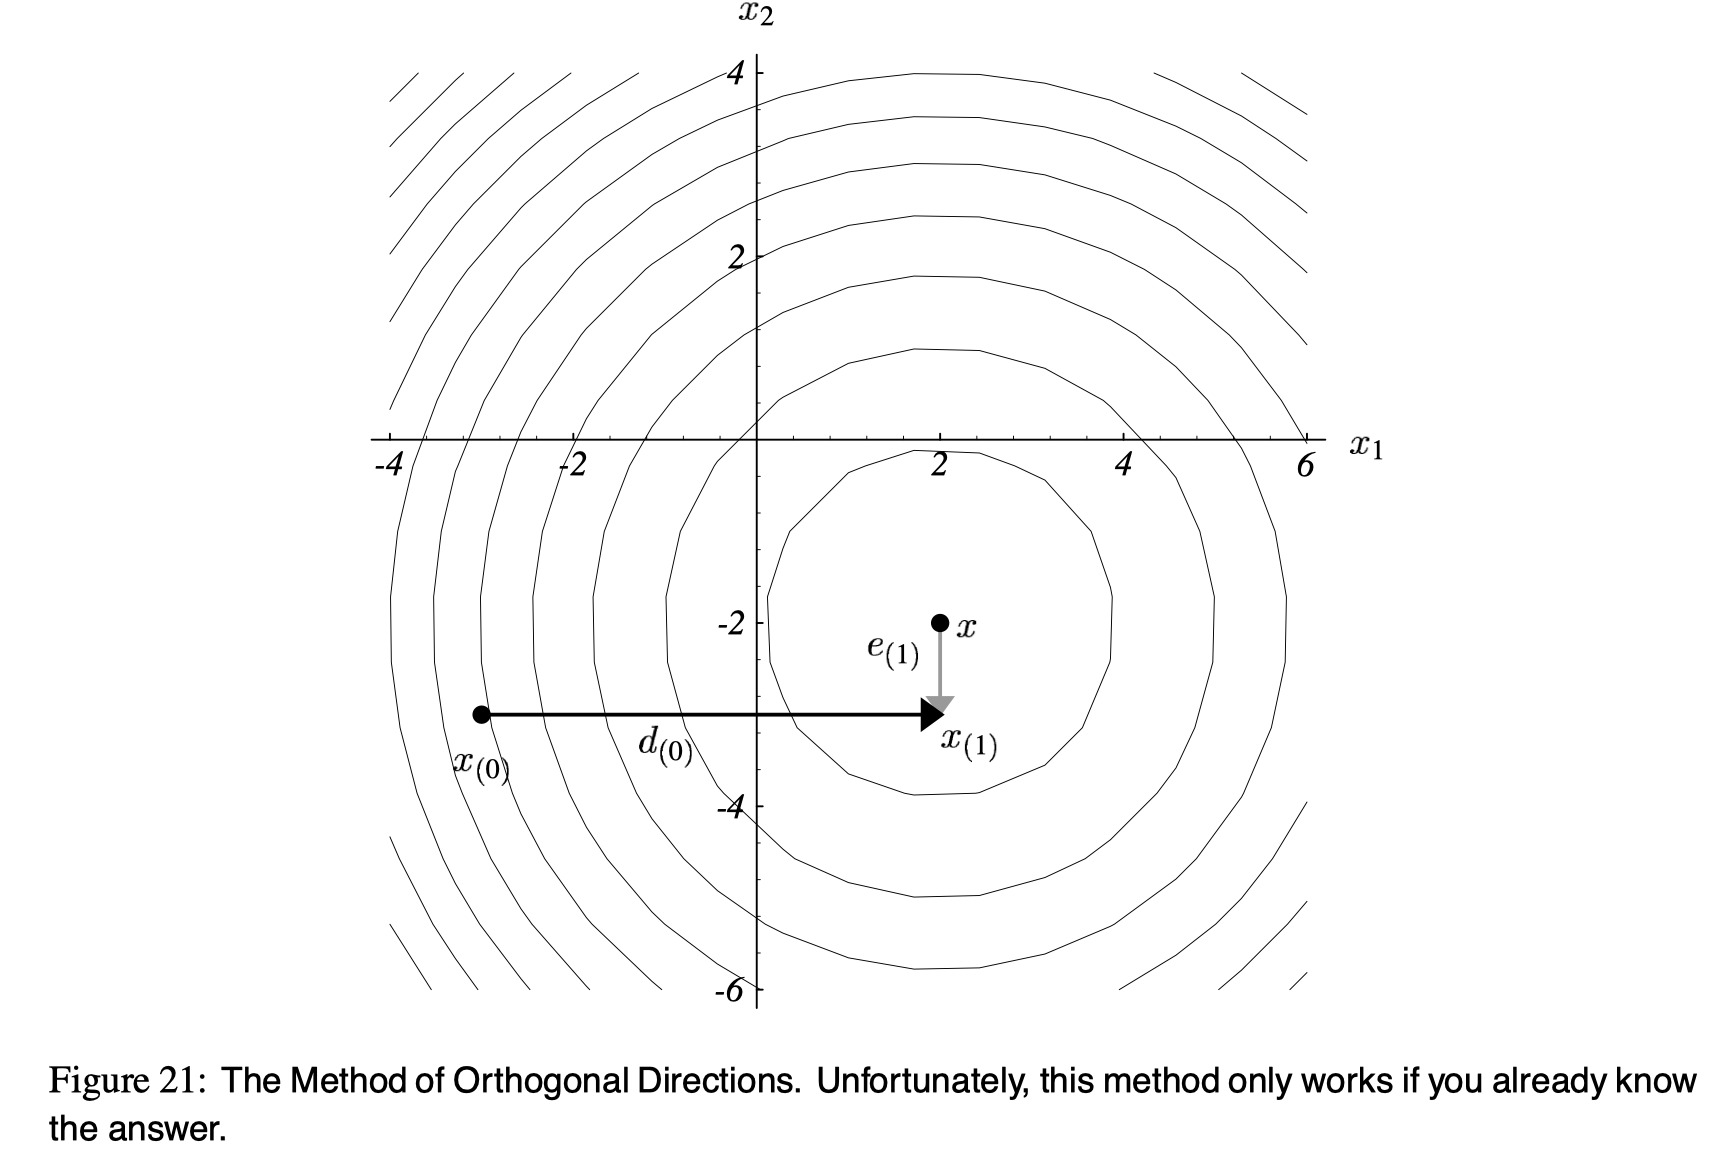
\includegraphics[width=1\textwidth]{fig/CG_Convergence_CD_1.png}
\end{figure}

为了确定 $\alpha_i$ 的值,需要注意到 $e_{i+1}$ 和 $d_i$ 是正交的,所以后续不能再重新回到 $d_i$ 的方向,因此有:
\begin{align*}
d^T_i e_{i+1} &= 0 \\
d^T_i(e_i + \alpha_i d_i) &= 0 \\
\alpha_i &= -\frac{d^T_ie_i}{d^T_id_i}
\end{align*}

但是显然,当前并不知道 $e_i$,所以也就无法确定 $\alpha_i$;

解决方法是,不是沿着相互正交(orthogonal)的方向搜索,而是沿着互相为 A-orthogonal 的方向搜索。

\textbf{如果两个向量 $d_i, d_j$满足如下条件;则称两个向量为为 A-orthogonal,或称 conjugate(共轭)}
$$
d_i^TAd_j = 0
$$

图22 示例了 A-orthogonal 的向量对(a) 和 orthogonal 的向量对(b)。
\begin{figure}[H]
    \centering
    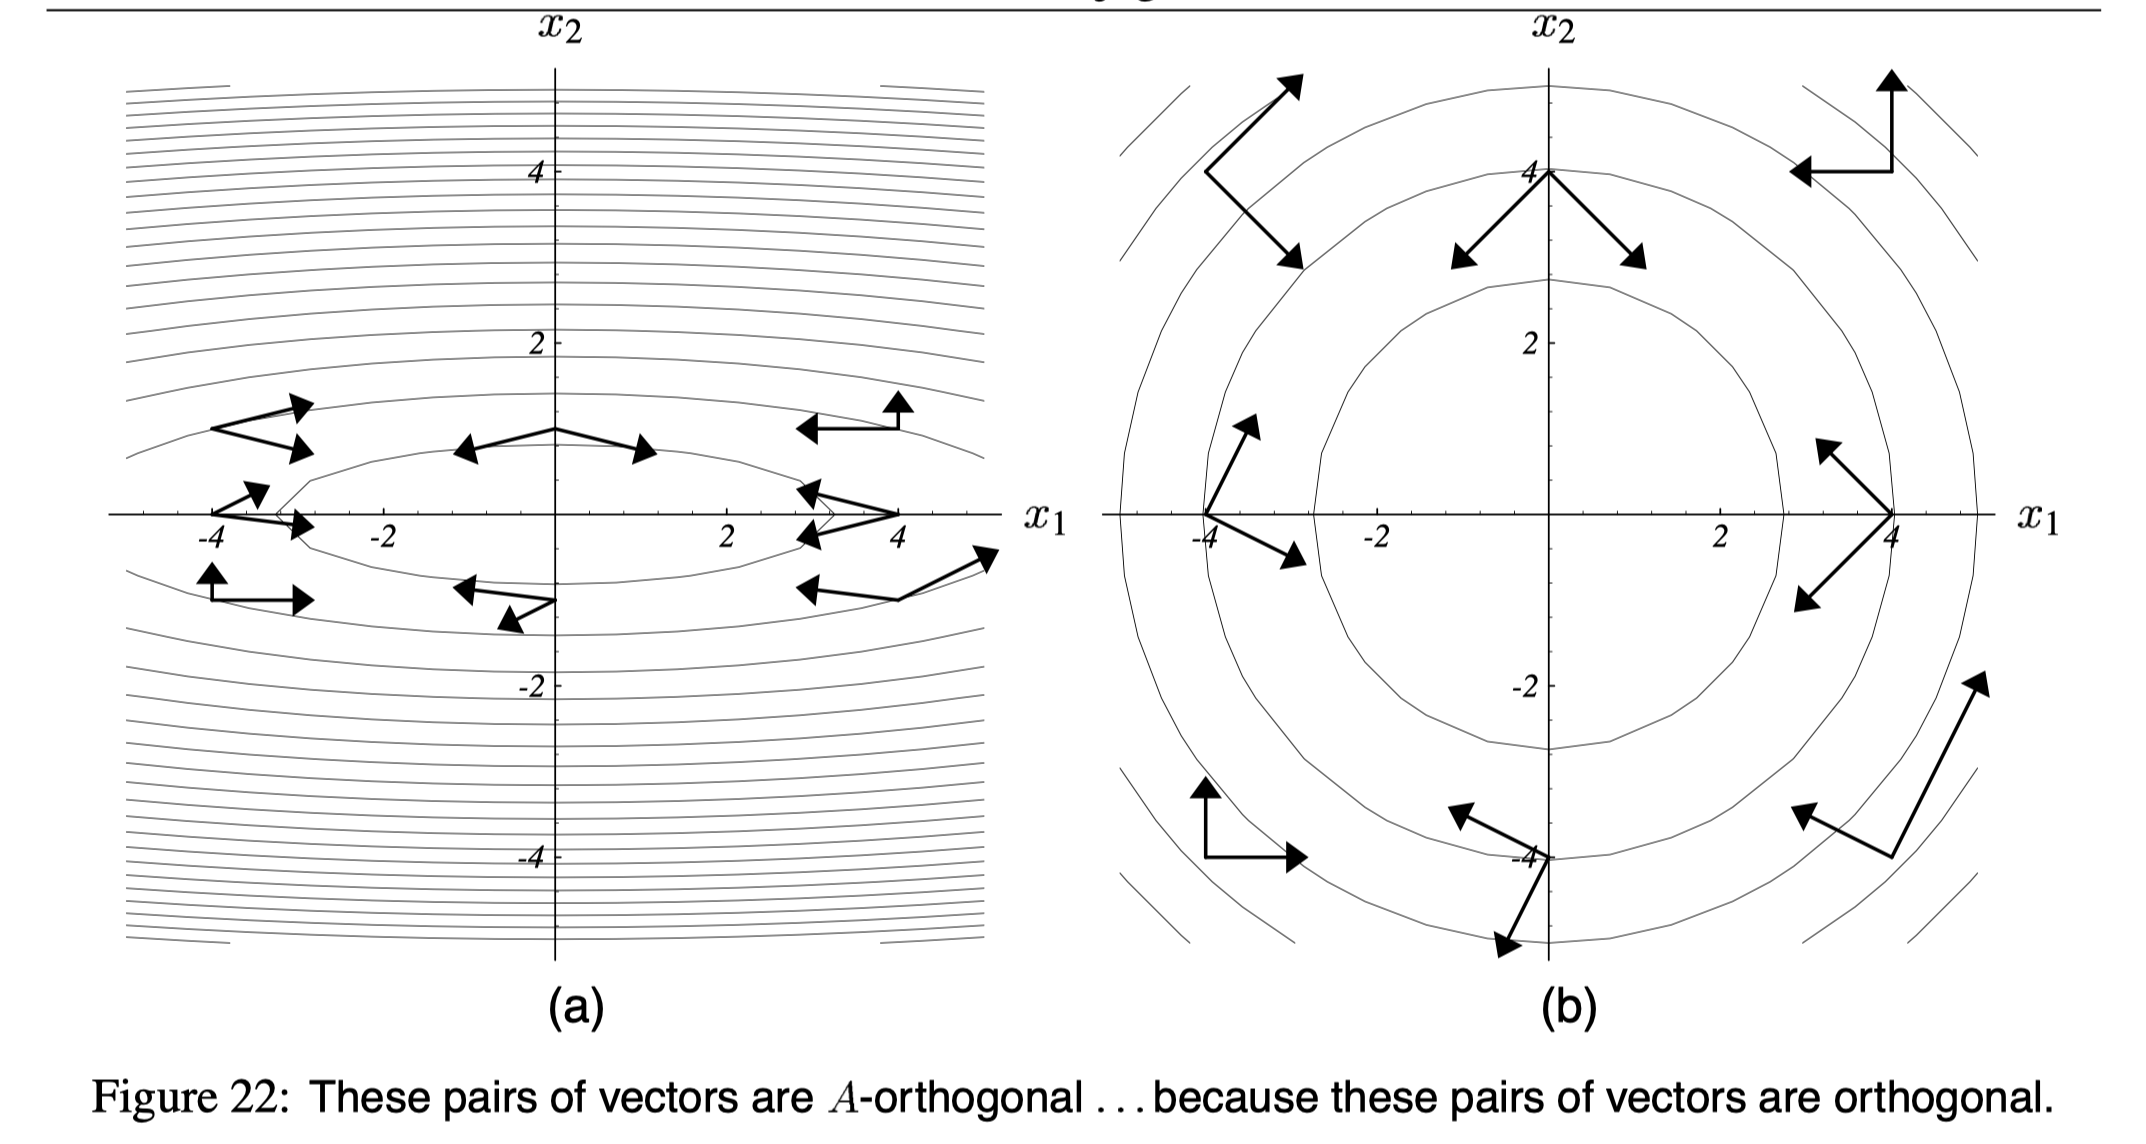
\includegraphics[width=1\textwidth]{fig/CG_Convergence_CD_2.png}
\end{figure}

接下来,我们令 $e_{i+1}$ 与 $d_i$ 满足 A-orthogonal,如图23(a) 所示。这个正交的条件等价于在 SD 算法中,沿着 $d_i$ 方向查找最小值点。证明如下:
\begin{align*}
\frac{d}{d\alpha}f(x_{i+1}) = 0 &\Rightarrow f'(x_{i+1})^T \frac{d}{d\alpha}x_{i+1} = 0 \Rightarrow \\
-r^T_{i+1}d_i &= 0 \\
d^T_iAe_{i+1} &= 0
\end{align*}

同理,根据上文确定 $\alpha_i$ 的方法,有:
\begin{align*}
d^T_iAe_{i+1} &= 0 \Rightarrow \\
d^T_iA(e_i + \alpha_id_i) &= 0 \Rightarrow \\
\alpha_i &= -\frac{d^T_iAe_i}{d^T_iAd_i} \\
	&= \frac{d^T_ir_i}{d^T_iAd_i}
\end{align*}
\begin{figure}[H]
    \centering
    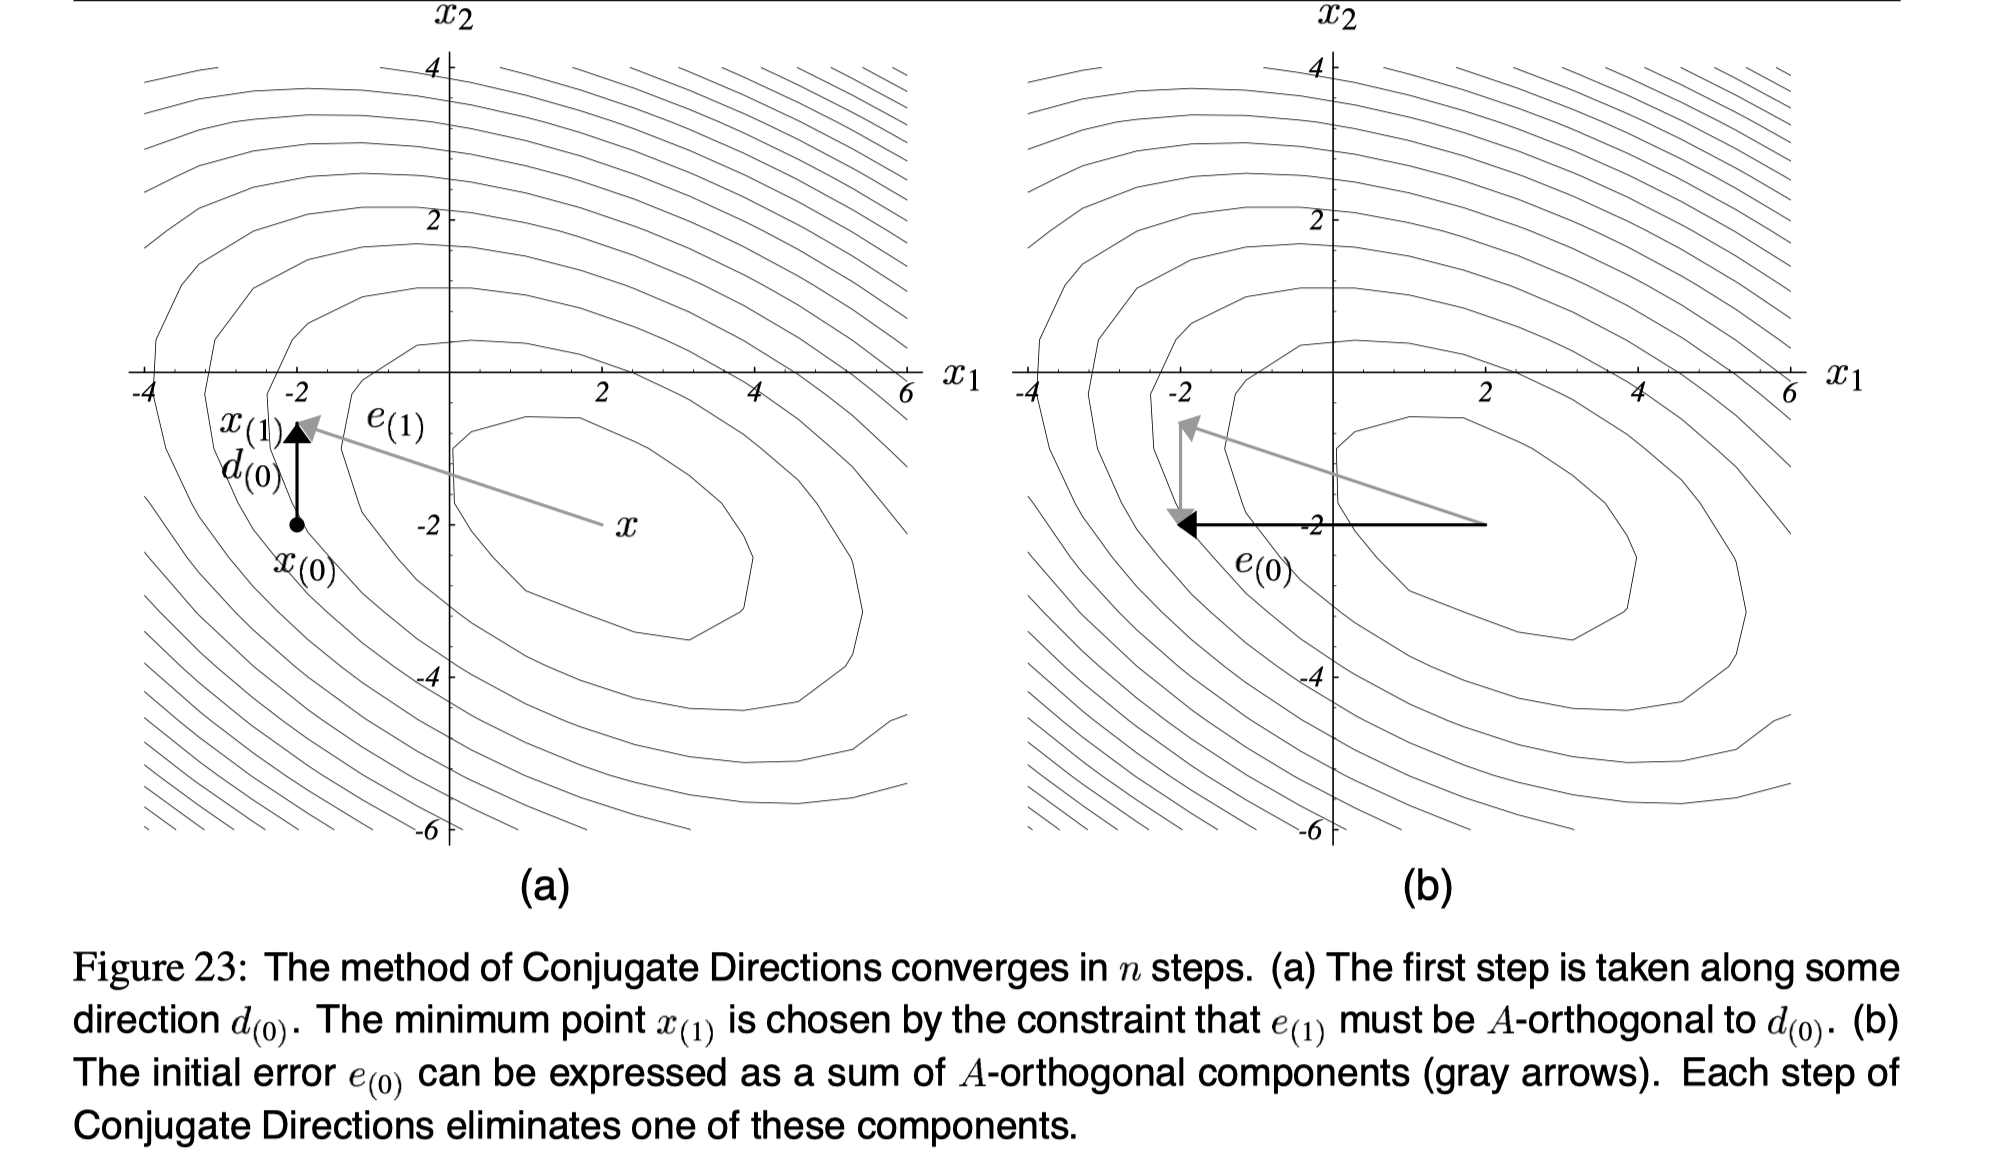
\includegraphics[width=1\textwidth]{fig/CG_Convergence_CD_3.png}
\end{figure}

\begin{framed}
\textbf{证明:共轭法可以保证在 $n$ 步内求得 $x$。}

首先,将误差 $e$ 表示为搜索方向的线性组合:
$$
e_0 = \sum_{j=0}^{n-1}\delta_jd_j
$$

接下来,使用数学上的小技巧,将 $\delta_j$ 消去到只剩下一项:
\begin{align*}
d^T_kAe_0 &= \sum_j\delta_jd^T_kAd_j \\
d^T_kAe_0 &= \delta_kd^T_kAd_k \qquad \text{(by A-orthogonality of d vectors)} \\
\delta_k &= \frac{d^T_kAe_0}{d^T_kAd_k} \\
	&= \frac{d^T_kA(e_0 + \sum_{i=0}^{k-1}\alpha_id_i)}{d^T_kAd_k} \qquad \text{(by A-orthogonality of d vectors)} \\
	&= \frac{d^T_kAe_k}{d^T_kAd_k} \\
\end{align*}

根据 $\alpha_i = -\frac{d^T_iAe_i}{d^T_iAd_i}$ 和 $\delta_k = \frac{d^T_kAe_k}{d^T_kAd_k}$ 可知,$\alpha_i = -\delta_i$。

然后,有:
\begin{align*}
e_i &= e_0 + \sum_{j=0}^{i-1}\alpha_jd_j \\
	&= \sum_{j=0}^{n-1}\delta_jd_j - \sum_{j=0}^{i-1}\delta_jd_j \\
	&= \sum_{j=i}^{n-1}\delta_jd_j
\end{align*}

也就是说,经过 $n$ 次迭代后,每一项都会减为 0 ,所以 $e_n = 0$,命题得证。
\end{framed}

\subsection{Gram-Schmidt 正交化(Gram-Schmidt Conjugation)}
接下来,通过 Gram-Schmidt Conjugation 法,能够生成一些列 A-orthogonal 的搜索方向集合$\{d_i\}$。

假定有 $n$ 个线性无关的向量 $u_0, u_1, \cdots, u_{n-1}$(简单的方法是选择坐标轴,但是接下来讨论更一般的方法),为了构造$d_i$,取$u_i$ 并且从之前的 $d$ 向量中,减去所有不满足 A-orthogonal 的分量(见图24)
\begin{figure}[H]
    \centering
    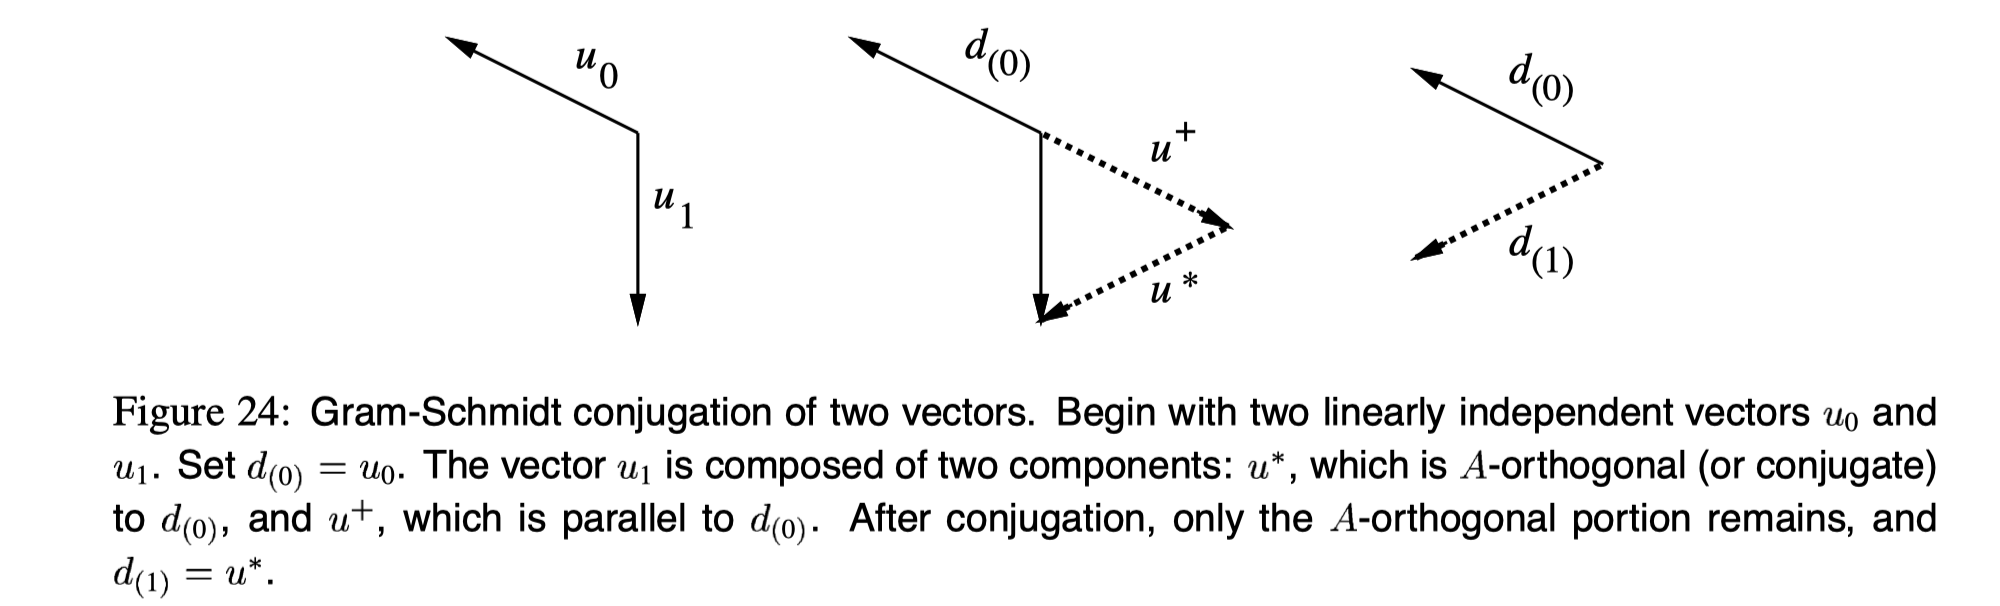
\includegraphics[width=1\textwidth]{fig/CG_Gram_Schmidt_Example.png}
\end{figure}

也就是说,令 $d_0 = u_0$,对于任意 $i > 0$,令:
$$
d_i = u_i + \sum_{k=0}^{i-1}\beta_{ik}d_k
$$

当 $i > k$ 时,$\beta_{ik}$有如下定义(和计算 $\delta_j$ 的trick相同):
\begin{align*}
d^T_iAd_j &= u^T_iAd_j + \sum_{k=0}^{i-1}\beta_{ik}d^T_kAd_j \\
0 &= u^T_iAd_j + \beta_{ij}d^T_jAd_j,  \qquad i > j \ \text{(by A-orthogonality of d vectors)} \\
\beta_{ij} &= -\frac{u^T_iAd_j}{d^T_jAd_j}
\end{align*}

使用 Gram-Schmidt 方法的困难点是需要将之前每步的搜索方向都存储下来,并且生成完整的搜索方向集合的复杂度是 $\mathcal{O}(n^3)$(?)。\textbf{如果使用坐标轴来生成搜索方向的集合,那该方法等价于高斯消去法(图25)}。所以该方法(Conjugate Direction)并不实用,直到发明了共轭梯度法(CG),并且共轭梯度法也是一种 Conjugate Direction 方法。
\begin{figure}[H]
    \centering
    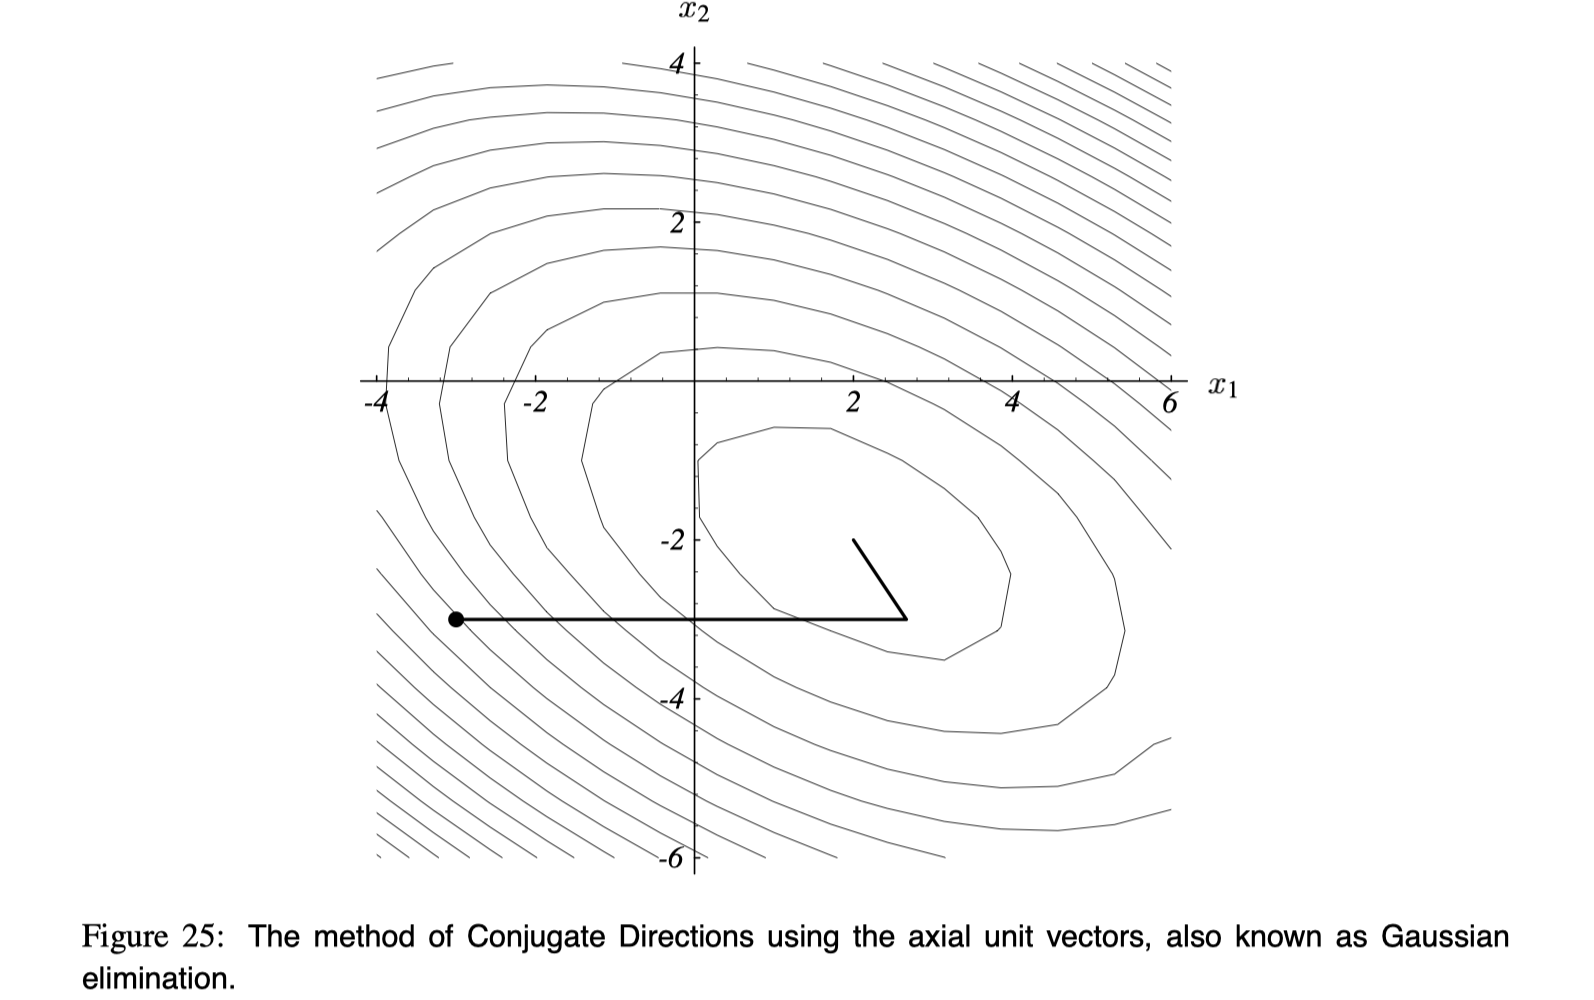
\includegraphics[width=1\textwidth]{fig/CG_Convergence_CD_4.png}
\end{figure}

对比图25和图21可以发现,图25就是拉伸版的图21。所以,当使用 Conjugate Direction 方法(和 CG 方法)时,就是在一个拉伸后的空间内使用 Orthogonal Direction 方法。

\subsection{误差项的最优化}
Conjugate Direction 方法有一个很好的性质:在允许的搜索空间内,每一步都在上界内找到最优解。(Conjugate Directions has an interesting property: it finds at every step the best solution within the bounds of Œwhere it’s span been allowed to explore.)

定义 $\mathcal{D}_i$ 为 $i-$维子空间($i$-dimensional subspace span $\{d_0, d_1, \cdots, d_{i-1}\}$;误差 $e_i$ 从 $e_0 + \mathcal{D}_i$ 中得到。找到最优解的含义是,在 $e_0 + \mathcal{D}_i$ 中选择能够最小化 $||e_i||_A$ 的解(见图26)。实际上,在空间 $e_0 + \mathcal{D}_i$ 中最小化  $||e_i||_A$ 也能推导出 CG 方法。
\begin{figure}[H]
    \centering
    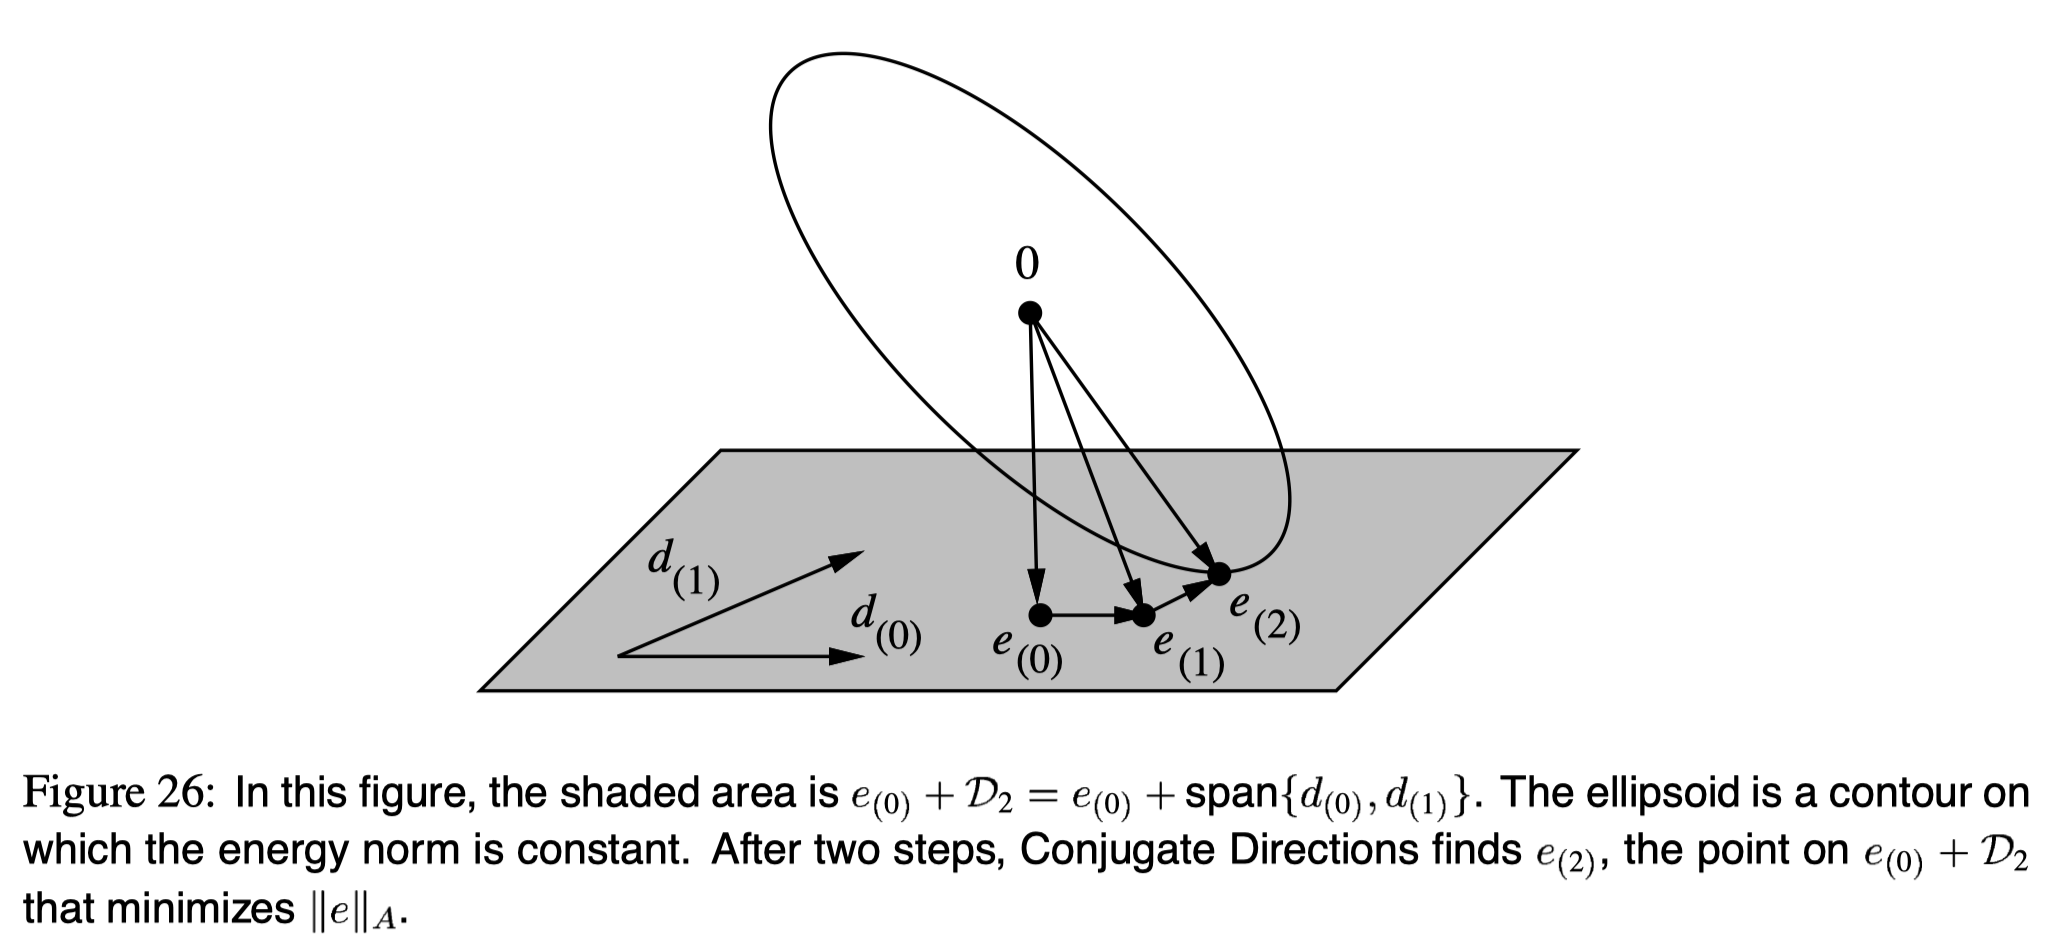
\includegraphics[width=1\textwidth]{fig/CG_Convergence_CD_5.png}
\end{figure}

按照之前将误差表示为搜索方向的加权和的方式,将 $||e_i||_A$ 表示为如下形式:
\begin{align*}
& \because e_i = \sum_{j=i}^{n-1}\delta_jd_j  \  \text{并且} \ ||e_i||_A = (e_i^TAe_i)^{1/2} \\
&\therefore ||e_i||^2_A = \sum_{j=i}^{n-1}\sum_{k=i}^{n-1}\delta_j\delta_kd^T_jAd_k = \sum_{j=i}^{n-1}\delta_j^2d^T_jAd_j\\
\end{align*}

其中每一项都和未进行的搜索的方向有关;任意从空间$e_0 + \mathcal{D}_i$中得到的误差 $e$ 都会有相同的扩展项,从而证明了 $e_i$ 一定最小化的 energy norm???。

图27(a)(c) 演示了 $\mathbb{R}^2$ 和 $\mathbb{R}^3$ 空间中的 Conjugate Directions 方法,图中看起来垂直的线是正交的;图27(b)(d) 对应在变形后的空间中(椭圆形变成圆形)图中看起来垂直的线是A-orthogonal 的。
\begin{figure}[H]
    \centering
    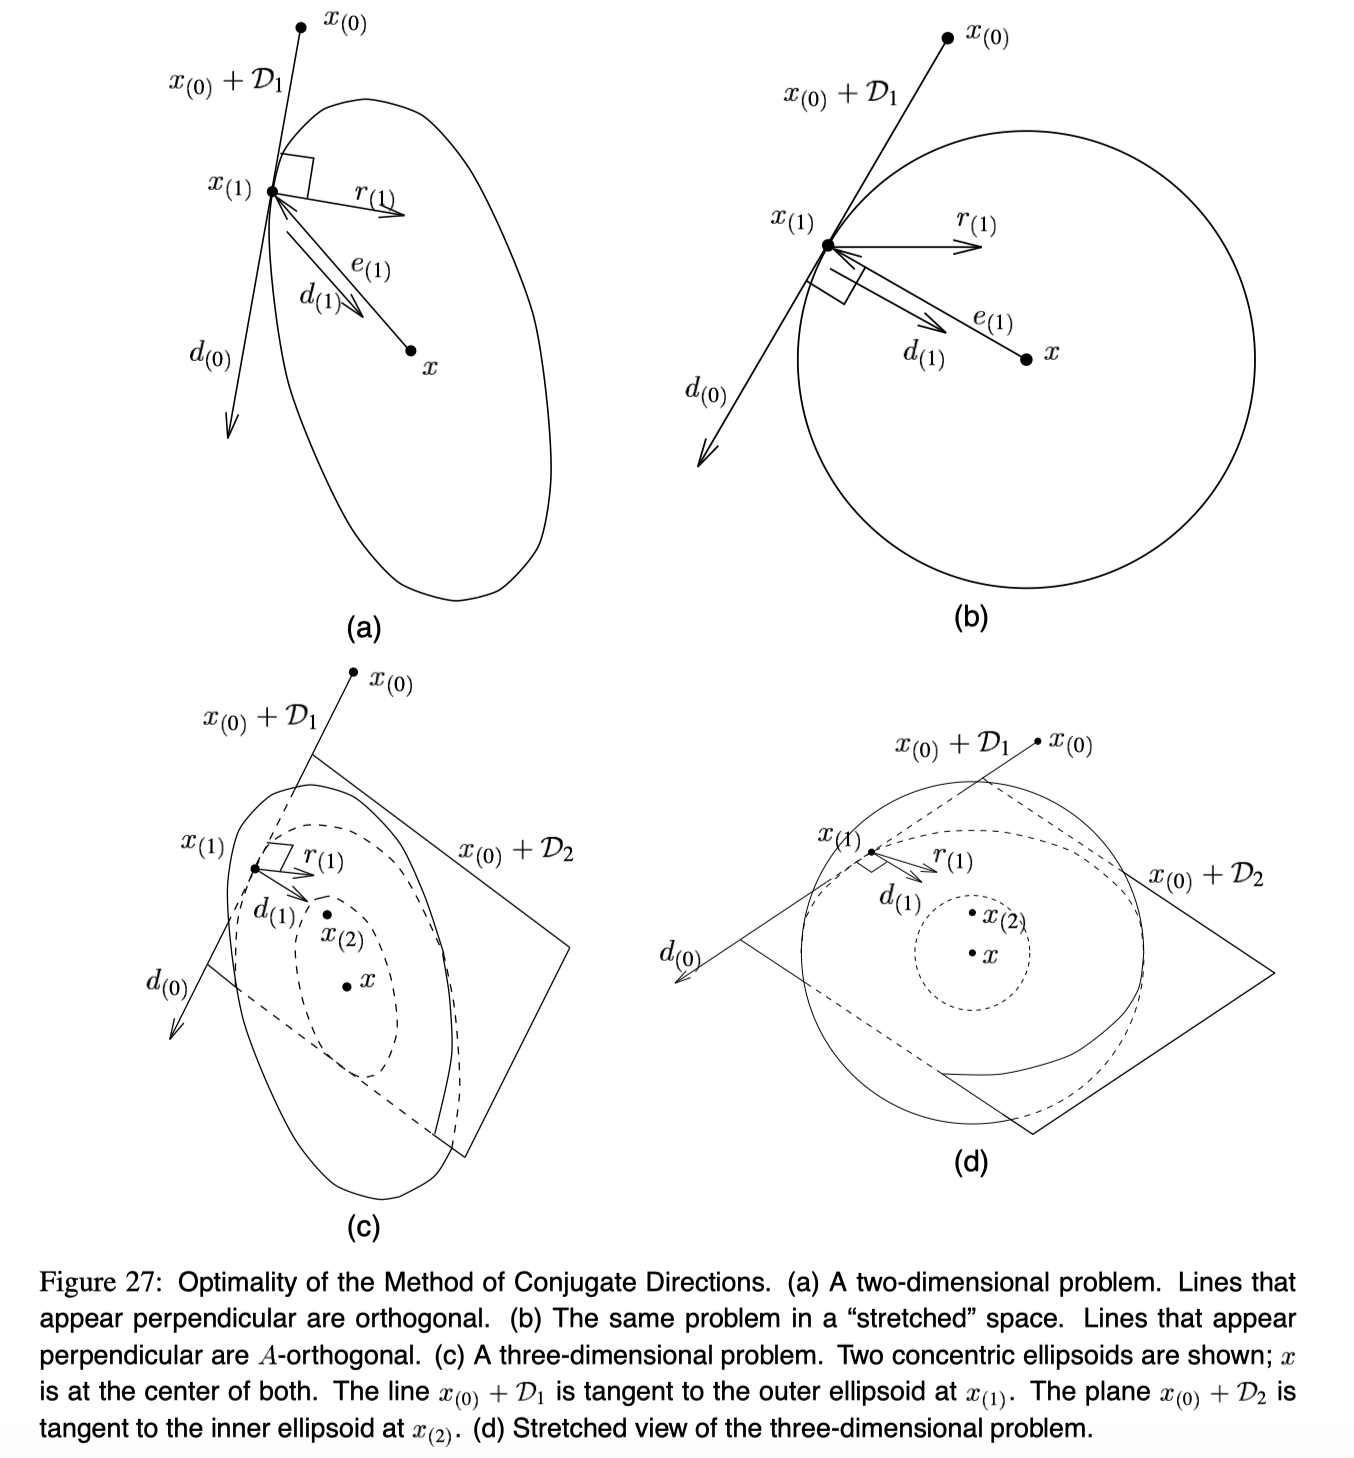
\includegraphics[width=1\textwidth]{fig/CG_Convergence_CD_6.png}
\end{figure}

在图27(a) 中,Conjugate Directions 方法从点 $x_0$ 开始,延 $d_0$ 方向经过一步,到达点 $x_1$,误差 $e_1$ 与 $d_0$ 是 A-orthogonal 的;为什么 $e_1$ 是空间 $x_0 + \mathcal{D}_1$ 中的最小解呢?从图 27(b) 可以看出来,在变形后的空间中, $e_1$ 与 $d_0$ 是垂直的。$e_1$是 $||e||_A$ 为常量时的同心圆的半径,所以 $x_0 + \mathcal{D}_1$ 与 $x_1$ 与该圆正切与点 $x_1$。所以 $x_1$ 是在 $x_0 + \mathcal{D}_1$ 空间中使得 $||e_1||_A$ 最小的点。

%\printbibliography
\bibliography{../ref}
\bibliographystyle{IEEEtran}
\end{document}

